\documentclass{kuee}
\renewcommand{\include}[1]{}
\renewcommand\documentclass[2][]{}
\usepackage[dvipdfmx]{graphicx}
\usepackage{amsmath}

\title{表現型特徴ネットワーク解析におけるGroup-In-a-Boxレイアウトの有効性評価}
\etitle{Evaluation of Group-In-a-Box layouts in the analysis of phenotype network}
\author{青山 望}
\eauthor{Nozomi Aoyama}
\professor{小山田 耕二 教授}
\course{京都大学大学院工学研究科}
\department{電気工学専攻}
\date{令和2年1月31日}

%----------------------------------------------------------------------
% ここは,「作成の手引き」で使われているマクロを定義している部分です.
% 通常の修論・卒論の作成時には,削除して下さい.
\def\BibTeX{{\rm B\kern-.05em{\sc i\kern-.025em b}\kern-.08em
    T\kern-.1667em\lower.7ex\hbox{E}\kern-.125emX}}
\def\JBibTeX{\leavevmode\lower .6ex\hbox{J}\kern-0.15em\BibTeX}
\ifx\JTeX\undefined
  \def\JTeX{\leavevmode\lower.5ex\hbox{J}\kern-.18em\TeX}
\fi
\makeatletter
\def\chapterhead#1#2{%
  \bgroup
    \LARGE \bf
    \setbox\@tempboxa\hbox{第 \lower0.1ex\hbox{#1} 章\hskip 10pt}%
    \begin{list}{}{%
      \topsep = 0pt \parsep = 0pt
      \labelwidth = \wd\@tempboxa \labelsep = 0pt
      \leftmargin = \labelwidth
    }\item[\box\@tempboxa] #2
    \end{list}%
  \egroup
  \vskip 10pt}
\makeatother
% ここまでマクロ定義部分
%----------------------------------------------------------------------

%%% 本文
\begin{document}
\maketitle      % 表題を出力
\begin{eabstract}   % 英文要旨を出力
This document briefly explains the usage of the \LaTeX{} style file
for KUEE bacheler thesis and master thesis.
\end{eabstract}
\tableofcontents    % 目次を出力

\chapter{序章}
\label{chap:intro}
生命は生化学現象を基盤とし、遺伝子やmRNA、タンパク質、表現型特徴などの異なるスケールで制御される複雑系からなる。
この生命現象を理解するためには、様々な現象を観測し、そのダイナミクスや異なるスケール感の相互作用を細かに観察する必要がある。
観測したデータから新たな知見を導き出すために、データ駆動型科学が行われている。
これは事前の仮設なしにデータからないが言えるのかを考え、科学的手法における仮設生成をデータに基づいて行うというアプローチである。
データ駆動型科学においては、対象となるデータをいかに可視化するかが重要となる。
効果的な可視化を用いれば、データ得られる仮設の信頼性は高くなり、データ解析の効率も向上すると考える。

近年では顕微鏡により計測された細胞の時空間胴体を自動的に観測するバイオイメージ・インフォマティクス技術が発達したことで、大量かつ複雑な生命科学データが取得されている。
こうしたデータを有効に解析することができれば、新たな生物学的知見を得ることができるだろう。
しかし、増え続けるデータに従来の手法で効果的に可視化するのは難しく、データに対応するため新たな可視化手法の開発も進んでいる。
バイオイメージ・インフォマティクスの進歩に合わせ、可視化技術も進歩させることが有効なデータ駆動型科学には不可欠だと考える。

線虫(C. elegans)は線形動物門双腺綱に属する体長1mmほどの糸状の生物である。
実験材料として優れた性質をもつことから、モデル生物として広く利用されている他、多細胞生物として最初に全ゲノム配列が解読された生物でもある。
我々の共同研究者である理化学研究所の生命科学者達は、C. elegansを用いて個体発生を制御する遺伝子ネットワークを明らかにしようとしている。
比較的単純な細胞構造を持つC. elegansの発生メカニズムが明らかになれば、人間のようなより複雑な多細胞生物の発生メカニズムの解明につながり、ひいてはガン研究や再生医療に大きな貢献ができるであろう。

理化学研究所の研究員達は、現在C. elegansの表現型特徴ネットワークから生物学的な因果関係を示唆する関係性を抽出することを目指している。
表現型特徴とはある生物の持つ遺伝子型を形質として示したものである。
複数の表現型特徴間の相関や因果関係を探ることで、発生のメカニズムを解き明かすこという研究である。
発生中の胚の細胞の胴体を4次元的に計測した顕微鏡画像を取得し、その動画像データに対して画像認識プログラムを適用して核の大きさ等の胚の表現型特徴を動態を計測する。
計測された表現型特徴間の相関を計算することで、表現型特徴間の関係性から図\ref{fig:example_phenotype}のような表現型特徴ネットワークが構築される。
ここで、ノードはそれぞれの表現型特徴を表し、エッジは表現型特徴の相関を表す。
このネットワークから表現型特徴間の繋がりを抽出したり、重要な表現型特徴を繋ぐパスを探索することで仮設生成を行っている。

図\ref{fig:example_phenotype}は各表現型特徴をその発現時期と発現する細胞を基にグループ分けしている。
一番左に1細胞期を配置し、その右は1細胞期から2細胞期への変移期、その右は2細胞期と横方向には表現型特徴の発現時期順にグループを配置している。
縦方向は細胞ごとにグループを分けており、4細胞期には細胞ごとに4つのグループが存在する。
このレイアウトは各グループを階層的に配置しているために、全体のグループ構造を把握するには適しているが、実際のネットワーク解析では有効ではないと考えられる。
というのも、このレイアウトにはノード間を繋ぐエッジの情報が介在していないからである。
グラフ描画の分野では、ネットワークの可読性に影響する様々な要素が報告されている\cite{harel2000fast,koren2003drawing,hachul2004drawing,giacomo}。
具体的には、グループを表現する箱のアスペクト比やエッジの交差数、エッジの長さなどがネットワークの可読性を左右する。
より良い解析を行うためにはより効果的なレイアウトによってネットワークを可視化する必要があり、またドメインからのそうしたニーズが存在する。

表現型特徴ネットワークに見られるノードのグループはコミュニティ構造と呼ばれ、この特徴を持つネットワークを複雑ネットワークと呼ぶ\cite{Newman:2010:NI:1809753,girvan2002community,newman2004detecting}。
グラフ描画の分野では複雑ネットワークを可視化するため様々なネットワーク可視化手法が提案されてきた\cite{Vehlow2017VisualizingGS,doi:10.1177/1473871612455749,saket2014group}。
こうした手法はそれぞれ異なる目的のもと提案されている。
例えば隣接行列はネットワークデータを可視化する手法の一つであり、ノードを適当に並べ替えられる、ノード間にエッジがあるかなどの判定が容易であるというメリットを持つが、一方で複数ノード間の繋がりが理解しにくい、ノードの配置に位置情報を反映できないなどのデメリットがある。
このように各可視化手法には向き不向きがあることから、表現型特徴ネットワークにもそれに適した可視化手法を用いることが必要である。

% コミュニティ構造を持つネットワークはノードのグループをいくつか持ち、同一グループ内では密な接続があり、異なるグループ間では接続は疎になる。
% これは表現型特徴ネットワーク以外でも共通である。
% 複雑ネットワークの例としてTwitterネットワークが挙げられる。
% ノードはユーザーを表し、ユーザー間のフォローやリツイートをエッジとして表現したものである。
% こうしたネットワークでは、トポロジーやユーザーの特徴によりをユーザーをいくつかのグループに分けることができる。
% 例えばユーザーの位置情報によりグループを分けた際、同一グループ内の繋がりは密であり、異なるグループ間の繋がりは疎であることが想像できる。

Vehlowらは複雑ネットワークを対象にした可視化手法に関する調査論文を発表している\cite{Vehlow2017VisualizingGS}.
Vehlowらは現行の手法をいくつかのカテゴリに分けて紹介している。
この中で、表現型特徴ネットワークはDisjoint flatのグループに入る。
これはノードが複数のグループに属さず、またグループ間に階層構造が存在しないというものである。
Disjoint flatなネットワークを可視化する手法にもいくつかの種類がある。
ノードの色で属するグループを表現するもの、グループ構造をネットワークと別に表すもの、グループ内のつながりを遷移行列で表すもの、グループ毎にノードを円や四角形で囲うものなどがある。
このうち、ノードの色でグループ構造を表すものはグループやノードの数が増えた際にカラーマップが難しくなるという欠点がある。
遷移行列を用いるものはグループ間の繋がりや複数ノード間の接続が理解しにくく表現型特徴ネットワークに適さない。
グループ毎に属するノードを図形で囲うという方法は、グループ構造のみならずエッジの情報など様々な要因を考慮してレイアウトができるため有効だと考えられ、Vehlowらも関連する研究を多数紹介している。

理化学研究所の研究員らなどの専門家は、これまで、表現型特徴ネットワークを可視化するのに同一グループに属するノードが四角形で囲まれているレイアウトを使用してきた。
こうした可視化手法はGroup-In-a-Boxレイアウト(GIB)と呼ばれ、そのうち4種類を図\ref{fig:example_GIB}に示す。
GIBは各グループに属するノードがノード数に比例した大きさの箱に囲まれており、グループ内のネットワーク、グループ間のネットワーク、グループの大きさを同時に表現できるという特徴がある。
図\ref{fig:example_phenotype}も各グループが箱に入っているが、箱の大きさがグループに属するノード数に対応しておらず、厳密にはGIBレイアウトではない。

GIBは表現型特徴ネットワークを表すのに適したレイアウトであるが、種類が多いためにどのレイアウトが一番有効であるか分かっていない。
いくつかの研究\cite{onoue2017optimal,chaturvedi2014group}で、計算的実験と小規模なユーザー実験によりGIBが評価されているが、我々の知る限りユーザー実験によりGIBを評価した研究は未だ存在しない。
上述したようにいくつかの計算可能な指標がグラフの可読性に影響することが分かっている\cite{harel2000fast,koren2003drawing,hachul2004drawing,giacomo}が、グラフの理解には人間の認知の観点からも様々な未解明の要因が影響するため、ユーザー実験を通した評価の必要性は高い。

以上のことから、我々は2種類のユーザー実験を行い、4種のGIBのうちどのレイアウトが最もデータ駆動型科学において表現型ネットワーク解析に有効かを検証する。
対象となるGIBは図\ref{fig:example_GIB}に示す4種類であり、順にST-GIB(Squarified-Treemap GIB), CD-GIB (Croissant-and-Doughnut GIB), FD-GIB (Force-Directed GIB), TR-GIB (Tree-Reordering GIB)である。
ST-GIBは箱の配置にsquarifiede treemapアルゴリズム\cite{bruls2000squarified}を使用している。
CD-GIBはグループにエッジで繋がっている他のグループの数に基づきグループを配置するものである、エッジの長さを短くして視覚的乱雑さを軽減する目的がある\cite{chaturvedi2014group}。
FD-GIBは各グループをノードとして捉え、グループの配置にforce-directedアルゴリズムを用いたものである\cite{chaturvedi2014group}.
TR-GIBは最適化問題を解いてエッジの長さの和が最小になるようにST-GIB内で箱を並び替えたものである。

一つ目の実験では、4種類のタスクを用いて様々な側面から4種類のGIBを評価することを目的とする。
二つ目の実験では、一つ目の実験で好成績を残した2つのレイアウトに着目し、より実際の解析作業に近いタスクとデータを用いることでどちらのレイアウトが最良であるかを明らかにする。

実験では、正答率と完了時間を計測することでレイアウト間の優劣を比較した。
これに加え、視線追跡システムを利用し実験中の被験者の視線データを記録した。
視線追跡システムは、ヒューマンコンピューターインタラクションの分野でよく用いられる。
実験中の視線データを解析することで、実験結果の優劣がなぜ生まれたかについて議論することができる\cite{andrienko2012visual,duchowski2007eye,kurzhals2014evaluating}。
具体的には、ネットワークグラフにおけるどの視覚特徴が被験者のパフォーマンスに影響したかを特定することを目指す。

本研究の主な有効性は4種のGIBを評価することでどのレイアウトが表現型特徴ネットワークの解析に最も有効かを明らかにすることである。
我々はGIBはその視覚的特徴の違いから、ユーザー実験の結果にも差が出ると考えている。
最良のレイアウトが明らかになれば、それを用いることで表現型特徴ネットワークの解析の効率化が測れるだろう。
有効性としてもう一点、視線追跡データを解析することにはより、ネットワーク可視化において可読性に影響し得る視覚的特徴を特定することが挙げられる。
こうした特徴を発見できれば、GIBや他のグラフ描画手法の可読性を向上させるアイデアを得られ、グラフ可視化手法の改善に貢献することができる。

また、本研究は表現型特徴ネットワークの解析効率化に動機づけられたものであるが、GIBは他の複雑ネットワークにも利用可能な手法である。
上述したTwitterのようなSNSネットワークの他、企業間取引ネットワークや交通ネットワークにも応用が可能である。
本研究で明らかになった最良のGIBはこうしたデータでも有効であると考えられる。


\begin{figure}
  \centering
  \label{fig:example_phenotype}
  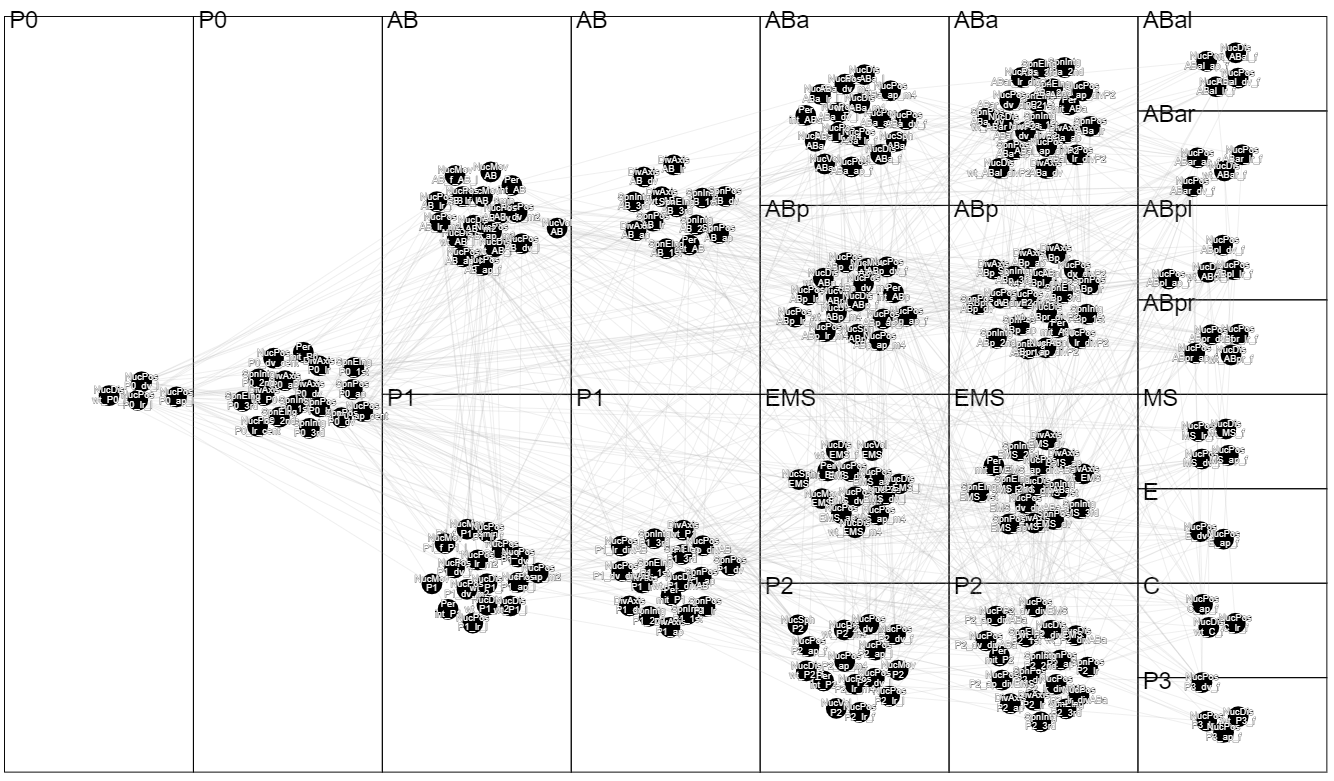
\includegraphics[width=15cm]{./images/PhenotypeNet.png}
  \caption{表現型特徴ネットワークの例}
\end{figure}

\begin{figure}
  \centering
  \label{fig:example_GIB}
  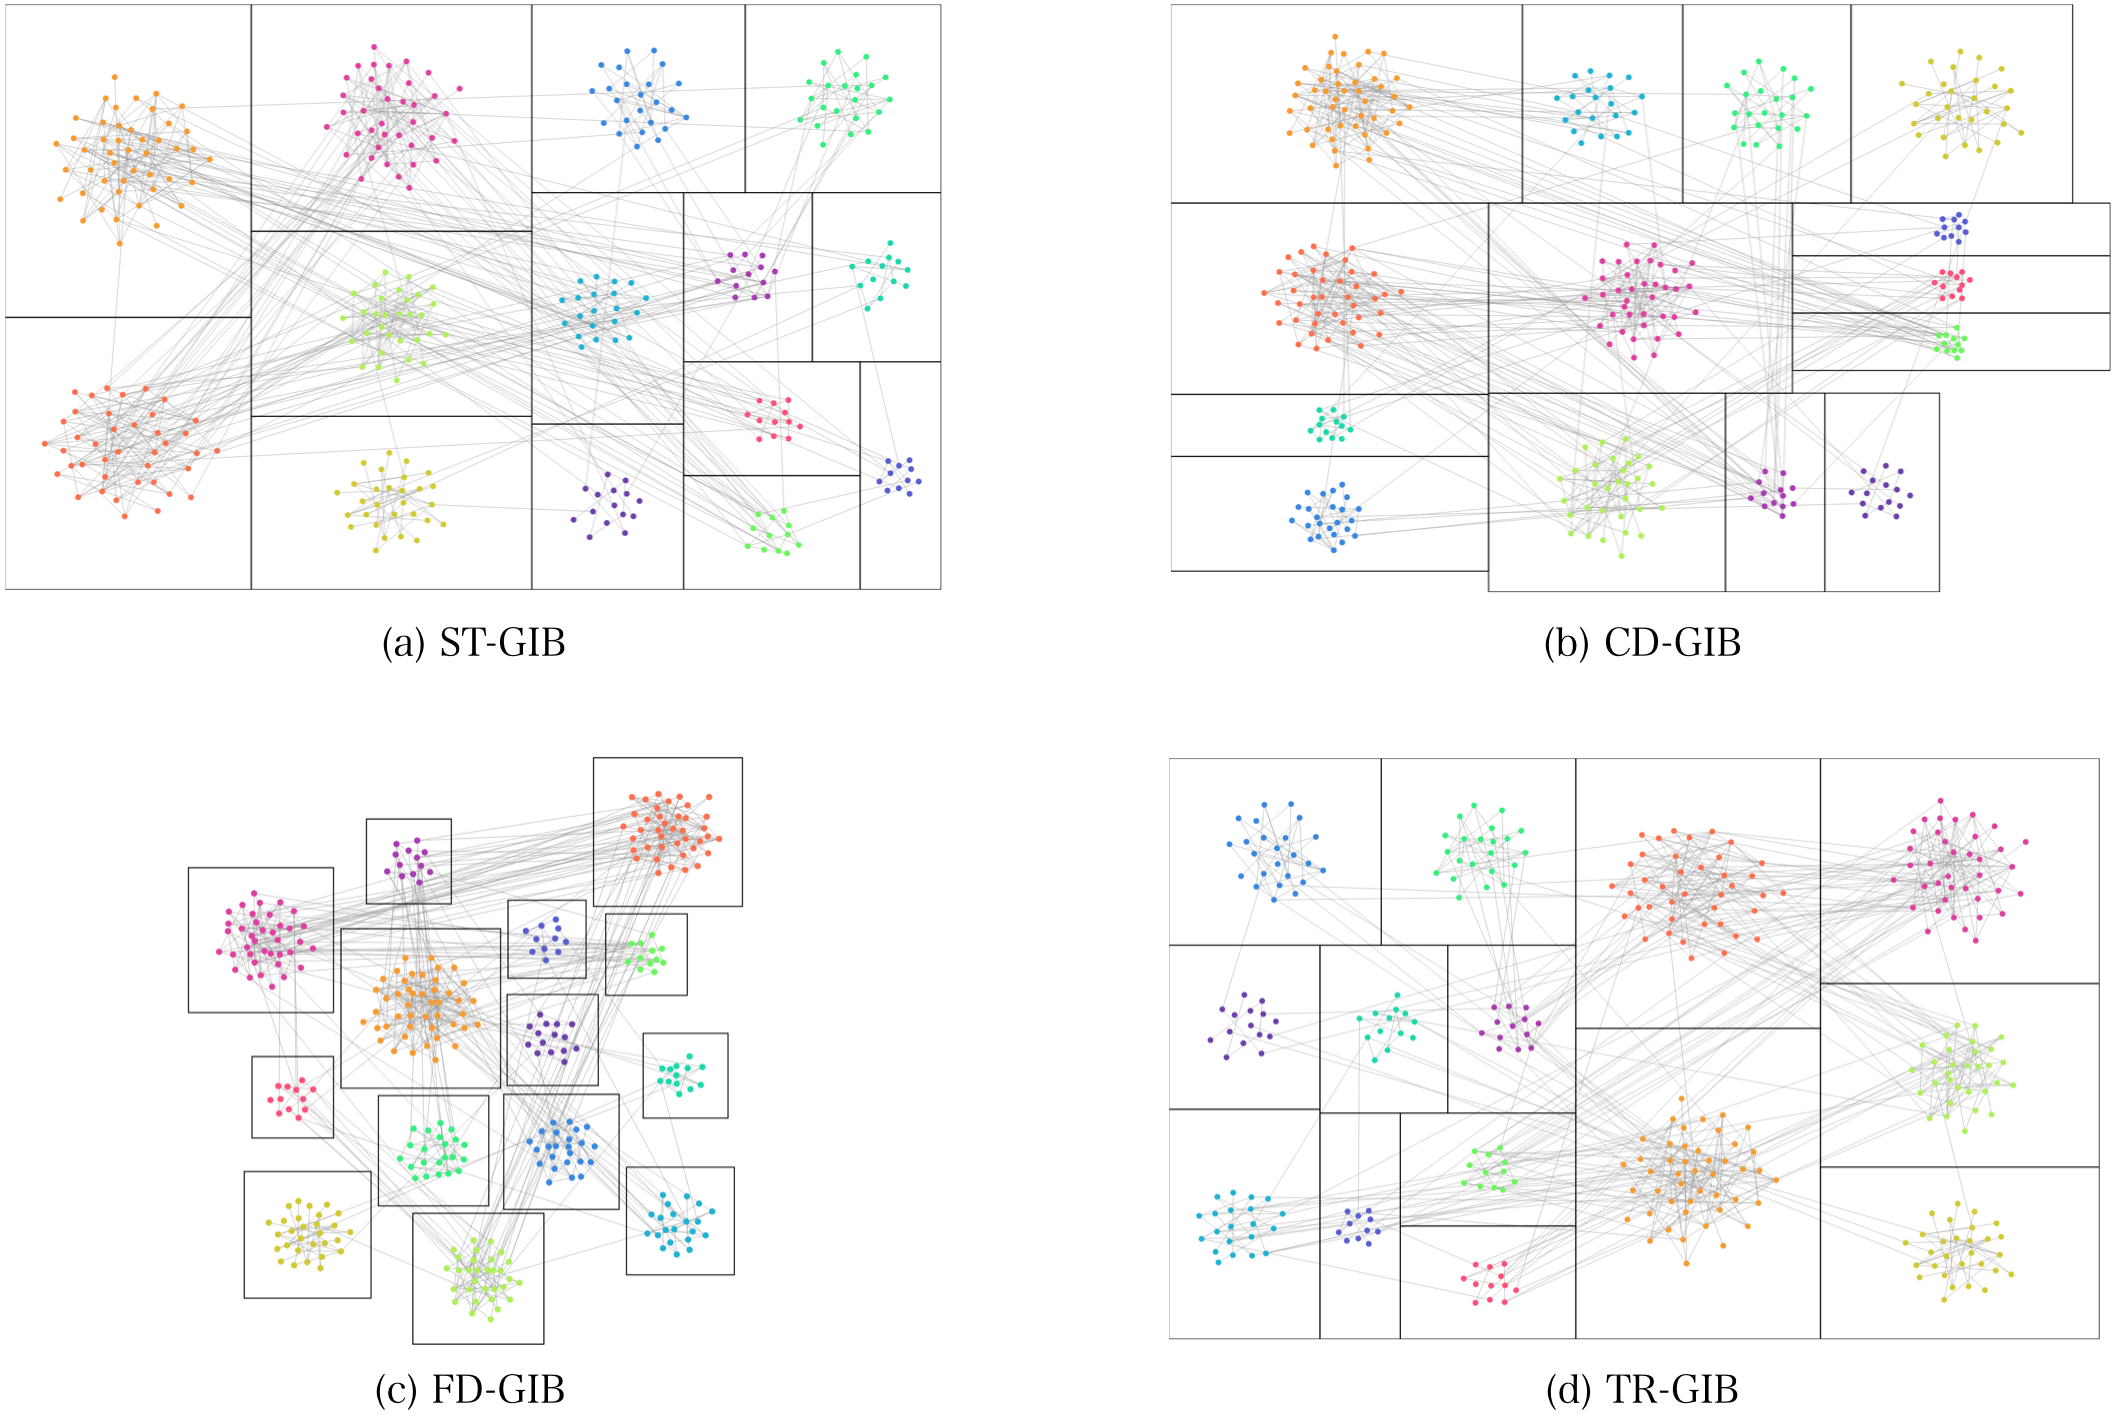
\includegraphics[width=15cm]{./images/examples.png}
  \caption{GIBレイアウトの種類。(a)ST-GIB, (b)CD-GIB, (c)FD-GIB, (d)TR-GIB}
\end{figure}


\chapter{関連研究}
\label{chap:relatedwork}

本章では関連研究について記述する。
本研究は生物学やグラフ描画、可視化の評価など様々な研究が関連するため、3節に分けてこれを述べる。
\ref{sec:vis_bio}節では生物学データの可視化について述べる。
特に、本研究は表現型特徴ネットワークの可視化に焦点を当てており、現在までの研究とその問題点について論述する。
\ref{sec:graph_for_group_structure}節ではグループ構造を持つネットワークの可視化手法について述べる。
こうした可視化手法にはいくつか種類があるが、その中でのGIBの立ち位置と、なぜGIBを研究対象にしたかを詳細に説明する。
\ref{sec:evaluation_with_eyetracking}節では視線追跡グシステムを用いた可視化の評価研究について記述する。
可視化の評価という分野は近年その重要性を高めているが、その中でも視線追跡システムを用いたものは結果をより定量的に述べられる上更なる考察を与えられるがために学術的な価値が高い。
一方で、高性能な視線追跡システムが一般に使用されるようになってから日が浅く、そのデータの膨大さから解析方法もあまり整っていない。
関連研究を詳細に述べることで、本研究の目的に即した視線データ解析を目指す。

\section{生物学データの可視化}
\label{sec:vis_bio}
顕微鏡により計測された細胞の動態を自動的に計測するバイオインメージ・インフォマティクス技術の発達により、大量の生命科学データが記録されている。
こうしたデータを解析するために、ImageJ\cite{schneider2012nih}に代表されるような取得された画像データを定量化し可視化する汎用的なツールも盛んに開発されている\cite{schindelin2012fiji,carpenter2006cellprofiler,Chen491035}

\section{Graph-drawing Method for Group Structure}
\label{sec:graph_for_group_structure}
データの重要性が広く認知されている近年では、頻繁なデータ収集や計測機器の進化によりネットワークデータはその量も複雑性も増している。
ネットワークの膨大さと複雑さに対応するため、グラフ描画の分野では様々な手法が提案されてきた。
Eadesらはforce-directed layoutと呼ばれる手法を提案した\cite{eades84}。
この手法では、ノード間の斥力とエッジ間の引力によって各ノードが配置される。
エッジが引力を持つことから、エッジにより繋がるノード同士が近くに配置され、エッジの長さが短くなる。
その計算的指標の優位性と見た目の美しさから、force-directedレイアウトは広く利用されいて\cite{Kobourov2013ForceDirectedDA}、かつこの手法にはにはいくつかの計算アルゴリズムが存在する\cite{harel2000fast,koren2003drawing,hachul2004drawing}。

一方で、グループ構造を持つ複雑ネットワークの可視化には専用に設計された可視化手法を用いるという動向がある。
大規模なネットワークデータでは、コミュニテイ検出の重要性は周知である。
複雑ネットワークの可視化にはいくつかの手法があるが、その多くはforce-directedレイアウトに基づいたものである。
グループ構造を表現する最も典型的な方法はノードを属するグループによって決まる色で描くものである\cite{mcpherson2005discovering}。
また、ノードの形をグループによって変化させるという方法も考えられる。
しかし、こうした方法は大規模な実際のデータでは効果的でないと知られている。

Vehlowらは複雑ネットワークの可視化手法に関する調査論文を発表している\cite{Vehlow2017VisualizingGS}.
彼女らは可視化手法自体とユーザー実験で用いられたタスクについて詳細に記述し、それぞれをいくつかのカテゴリに分類している。
可視化手法の分類は可視化手法とデータの構造の特徴により決まる。
前者はグループ構造が視覚的にどう表現されているかを表しており、その表現の仕方によってノード属性、並置、上書き、埋め込みという4つの分類に分けられる。
後者はグループの重複性とグループ間の階層構造性が基準となる。
ノードは同時に複数のグループに属することもあり、これの有無がグループの重複性となる。
ある2つのグループの中に包含関係があることもあり、これの有無が階層構造性となる。
Vehlowらは今までに提案された複雑ネットワーク向けの可視化手法のそれぞれのカテゴリに分けて紹介している。

GIBレイアウトも複雑ネットワークを可視化視する手法の一つである\cite{rodrigues2011group,chaturvedi2014group,onoue2017optimal}。
GIBには主に4つの種類(ST-GIB, CD-GIB, FD-GIB, TR-GIB)があり、本研究ではこれらを対象として比較実験を行う。
GIBはそれぞれのグループにスクリーン画面を割り当てて別箇に描画できるため、同一グループ内のネットワークを観察することが容易になる。
またグループを囲う箱の面積がグループに属するノードの数に比例しているため、グループの大きさも表現することができる。
Vehlowらの分類においては、当手法は上書き、重複性無し、階層構造性無しというカテゴリに分類される。
重複性無し、階層構造性無し、という性質の複雑ネットワーク向けにはいくつかの手法が紹介されている\cite{chaturvedi2014group,henry2007nodetrix,shneiderman2006network,bach2013graphdiaries,dekker2001visualisation}。
この内グループ情報の符号化に色のみを用いるものや、グループ情報をネットワークと分離して表現するものはGIBよりも効果的でないと考えられる。
遷移行列を用いたものは本研究の意義に沿わない。
同一グループを図形で囲う上書き方式が有効であり、その中でも計算的にグループの配置を調整しやすい四角形で囲んだもの、即ちGIBが一番有効であると考える。

少なくとも4種類あるGIBのうちいくつかは、計算的指標により評価がされている。
ChaturvediらはST-GIB, CD-GIB, FD-GIBの三種を309のTwitterネットワークを用いて、エッジと箱の交差数、スクリーン画面の使用効率、計算時間、平均の箱のアスペクト比を計算することにより比較した\cite{chaturvedi2014group}。
またその予備実験としてST-GIBとCD-GIBを9人の被験者を用いて4つのタスクにおいてその使いやすさを0 - 9のスコアで被験者に評価してもらった。
予備位実験ではCD-GIBの方が使いやすいという結果が出ている。
計算実験では三種類のレイアウト間で優位な差が確認されている。
FD-IGBはエッジと箱の交差数が少ないという利点があったが、スクリーン画面を浪費していた。
CD-GIBは計算時間が短く、ST-GIBはスクリーン画面の使用効率がよかった。
しかし、予備実験はタスクにおいて精度などの指標を用いてない他、計算実験では多数のエッジを一本にまとめて描いたグラフを使用していて信頼性に欠けるなど、評価の点では問題がある。
尾上と小山田はTR-GIBの有効性を示すため、計算によりTR-GIBによりグループの近接性(重み付けたエッジの長さの総和)が小さくなることを示しているが、他手法と比較したわけではなくユーザー実験も行っていない\cite{onoue2017optimal}。

計算指標による可視化の有効性評価は効果的であるが、グラフの可読性は複雑な人間の認知の観点からも考える必要があり、手法の有効性を根拠づけるには不十分である。
複数レイアウトを用いて被検者に特定のタスクを行わせるユーザー実験を行うことで、レイアウトの有効性をより実践的に評価することができる他、人間の認知といった計算では網羅できない観点も考慮することが可能となる。
DidimoとMontecchianiはforce-directed レイアウトに基づく良いGIBレイアウトを提案しているが\cite{6295786}、可視化結果が今回対象となるFD-GIBに酷似しているため、今回の実験対象からは外している。


\section{視線追跡システムによる可視化の評価}
\label{sec:evaluation_with_eyetracking}
視線追跡システムは視線データとユーザーの注意点を記録するため、ヒューマンコンピューターインタラクションの分野で広く用いられている\cite{andrienko2012visual,duchowski2007eye,kurzhals2014evaluating}。
可視化の評価に視線追跡システムを用いた研究はいくつかある\cite{burch2011evaluation,pohl2009comparing,netzel2014comparative,jianu2014display,7539393}。
こうした研究では、ユーザー実験中に視線データを記録ことで被験者がスクリーンのどの部分に注目しタスクを行なったかを議論している。
視線追跡データを解析することにより、実験で観測された差が生まれた理由についての糸口が得られる。

Burchらはツリーダイアグラム可視化手法の3種類を視線追跡システムを用いて評価した\cite{burch2011evaluation}.
彼らは与えられたノードの最低次共通親ノードを探すというタスクを探すというタスクを用いてユーザー実験を行なった。
実験中は正答率と完了時間に加え視線追跡データが記録され、Burchらは様々な手法をもって視線データを可視化し解析を行なった。
可視化には、軌跡マップやヒートマップ、関心領域(AOI)間の視線フロー図などが用いられた。
AOI(Area of Interest)は生命科学分野でよく用いられる考え方で、画像中の特定の領域に符号を割り当てたものである。
実験中にAOIを割り当てることで各AOI毎にデータ分析が可能になる。
視線追跡データを解析することにより、Burchらは異なる可視化手法間でタスク結果が異なった理由について考察している。
正答率が一番低かったレイアウトにおいては被験者が頻繁にクロスチェックをしていて、解答に迷っている様子が観察された。

こうした解析方法についてガイドラインを提供している研究もある\cite{andrienko2012visual,kurzhals2014evaluating,duchowski2007eye}.
時空間的スケールを持つ視線追跡データは量が膨大であり、解析にも特殊な方法を要する。
Burchらは視線データを解析する方法には二つの種類があると言及している\cite{Burch2013VisualTS}.
一つはAOIに基づいたもので、二つ目は視線の軌跡に基づいたものである。
ユーザーは興味のある領域や情報的に有益な領域に集中するがために、AOIが視線データ解析に重要だという事は古くから知られていた\cite{yarbus1967eye}.
GIBはスクリーンにいくつかの箱を配置する。
これらの箱は自然とAOIの役割を果たすため、本研究においてAOIに基づいたアプローチは視線データ解析に有効であると考える。
本研究ではGIBレイアウト間でユーザー実験に差が出た理由を明らかにするために視線追跡システムを用いる。

\chapter{GIB Layouts}
\label{chap:GIBs}

本章では評価の対象となる4種類のGIBについて記述する。
図\ref{fig:example_GIB}は対象となるGIBの例を示したものである。
図\ref{fig:example_GIB}の各図はレイアウトは異なるものの同じネットワークデータを可視化したものである。
これらのレイアウトはChaturvediら\cite{chaturvedi2014group}と尾上及び小山田\cite{onoue2017optimal}がいくつかの計算的指標によって評価したものであるが、レイアウトの有効性は計算指標のみでは測れるものでは無く、ユーザー実験の必要性は依然として残っている。

\section{ST-GIB}
Squarified-Treemap GIB (ST-GIB) (図\ref{fig:example_GIB} (a)はRodoriguesらによって提唱された物であり、Brulsによって提唱されたSquarified Treemapアルゴリズムに基づいたものである\cite{bruls2000squarified}.
Brulsらのアルゴリズムは元々ツリーマッピングに向けたものであった。
ツリーマッピングとは、スクリーン画面のサイズとデータ列を入力として、スクリーン画面をデータに比例する面積を持つタイルに分割する方法である\cite{shneiderman1992tree}.
ST-GIBは各グループをツリーにおける頂点と捉え、Squarified Treemapアルゴリズムによって画面を分割し、それぞれのタイルにグループ毎のネットワークを描画することによって生成される。

ツリーマップ法はスクリーン画面を効率的に活用できる上、それぞれの箱のアスペクト比が1に近いため、箱の中に描画されている各グループ内のネットワークが理解しやすいとされている\cite{bruls2000squarified}。
ST-GIBは箱の配置をSquarified Treemapアルゴリズムに依存しているが、この方法では各グループに含まれるノードの数のみが影響し、ノードを繋ぐエッジの情報が考慮されていない。
そのためエッジが長くなったりエッジの交差数が増えるといったネットワークグラフの可読性を下げる要因が観測されている\cite{468391,purchase1997aesthetic,purchase1998performance,purchase2002empirical}.
ST-GIBの実装にはBrulsらの手法を用いたsquarify Python ライブラリ (https://github.com/laserson/squarify)を使用した。
この手法では箱をその大きさの順で並べるために、被験者は箱の大きさを容易に比較することができると期待される。

\section{CD-GIB}
図\ref{fig:example_GIB} (b) に示されるCroissant-and-doughnut GIB (CD-GIB)はChaturvediらによって提案された\cite{chaturvedi2014group}ものである。
これはグループ間をまたがるエッジの情報を追加することにより、ST-GIBのエッジの情報が考慮されていないという欠点を克服しようとしたものである。
具体的には、G-degreeとG-skewnessの二つの指標によりCroissant-GIBレイアウトかDoughnut-GIBレイアウトのどちらかを選びタイルを配置する。
グループのG-degreeはそのグループがエッジにより繋がっている他のグループの数にと定義される。
また、全ノード数に対する最もG-degreeが高い2つのグループに含まれるノードの数の割合をG-skewnessとする。
これらの指標を用い、以下の基準でレイアウトを決定する。
\begin{itemize}
  \item Case1: G-degree $\ge$ or G-skewness $<$ 0.1: ST-GIB
  \item Case2: G $>$ 3 and 0.1 $\le$ G-skewness $\le$ 0.45: Doughnut-GIB
  \item Case3: G $>$ 3 and G-skewness $>$ 0.45: Croissant-GIB
\end{itemize}
Chaturvediらは実験的にこの基準を決め、我々も同様にこれを用いた。

Croissant-GIBではまずG-degreeが最大のグループをスクリーン画面の中央上部に配置する。
他のグループはG-degreeの大きい順に最初に配置したグループの周りを取り囲むように配置される。
結果として最初に配置した箱以外がクロワッサンのよう三日月型を形作るため、Croissant-GIBレイアウトと呼ばれる。
Doughnut-GIBでは最大G-degreeを持つグループをスクリーン画面の中央に配置する。
他のグループはCroissant-GIB同様にG-degreeの大きい順に最初には配置したグループを取り囲むように配置され、円形を形作るため
Doughnut型となる。

これらのこれらのレイアウトでは、他のグループとの接続が多いレイアウトがスクリーン画面の中央付近に配置されるため、エッジの長さが短くなり交差数が減り、ST-GIBよりも高い可読性が期待できる。
しかし、箱のアスペクト比が1から遠く、グループの大きさを推測するのが難しい他グループ内部のネットワークの表現に適していないと思われる。

\section{FD-GIB}
図\ref{fig:example_GIB}(c) に示されるForce-Directed GIB (FD-GIB) もまたChaturvediらにより提案された手法である。
このレイアウトでは、まず各グループをノードと捉え、それらがグループ間にまたがるエッジにより繋がっているネットワークを想定し、それをforce-directedレイアウトにより描画する。
このようにして各グループの位置を決めた後、グループを表す箱をその中心がforce-directedレイアウトにより配置された対応するノードの位置に一致するよう配置され、
その後箱の内部にグループ内部のネットワークが描画される。
このアルゴリズムでは箱が重なってしまうこともあり、これはPRISM法により取り除かれる\cite{gansner2008efficient}.

Force-directedレイアウトによりグラフを描画する方法にはいくつかの種類がある。
ChaturvediらはHarel--Koren fast multiscaleレイアウト\cite{harel2002graph}を使用したが、我々はD3.js force simulation\cite{Bostock:2011:DDD:2068462.2068631}を使用した。
これは可用性を考慮したが故であるが、Harel--Korenらの方法同様に良い結果が出ると知られている。
しかし、Chaturvediらが述べているように\cite{chaturvedi2014group}、Hachulらの
実験\cite{Hachul:2005:ECF:2102325.2102348}により他にも高次元埋め込み法\cite{harel2002graph}や代数的マルチグリッド法\cite{koren2003drawing}など良い手法があると確かめられている.

Force-directedレイアウトは複雑ネットワークに向けたものではないが、エッジの短さやトポロジーの見やすさなど様々な利点を持つと言われる\cite{Kobourov2013ForceDirectedDA}。
FD-GIBでも同様の効果が期待でき、特にグループ間のネットワークを表現する機能は高いと思われる。
また、箱のアスペクト比を1に保つことができるため、グループ間の大きさを推定するのも容易だろう。
しかし、他手法に比べスクリーン画面の使用効率が悪く箱が小さいため、グループ内部のデータ解析では劣ると考えられる。

\section{TR-GIB}
Tree-Reordering GIB (TR-GIB) (図\ref{fig:example_GIB} (d))は尾上と小山田により提唱されたレイアウトである。
ST-GIBはツリー構造をタイルとして二次元スクリーンに描画するツリーマップに基づいたものである。
ツリーマップはツリー構造を保っているために、ツリーにおける同階層のタイル同士は並べ替えることができる。
ST-GIBにおいても、同様に並び替えることのできるタイルがある。
TR-GIBはこの特性を利用したもので、ST-GIBにおいてタイルの並び替えを行い、エッジの長さを短くしたものである。
具体的には、グループ近接性を最小化する最適化問題を問題を解く事によりこれが得られる。
グループ近接性は、異なるグループ間をの距離をそのグループ間に跨るエッジの本数で重み付けしたものの総和と定義され、式\ref{eq:group_proximity}と表される。
\begin{equation}
\label{eq:group_proximity}
  \sum_{t_1 \in C}^{} \sum_{t_2 \in C}^{} w_{t_1 t_2}(d_{t_1 t_2}^x + d_{t_1 t_2}^y)
\end{equation}
ここで、$C$はグループの集合、$w_{t_1 t_2}$はグループ$t_1, t_2$を跨るエッジの本数、$d_{t_1 t_2}^x, d_{t_1 t_2}^y$はそれぞれグループ$t_1, t_2$間の距離の$x, y$成分である。
これを最小化する事で、エッジの長さが短いレイアウトが得られる。

エッジの長さが短いと、交差数が少なくなるためTR-GIBは高い可読性が期待される。
また、このレイアウトはST-GIBの特徴も依然として保っていて、箱のアスペクト比が1に近くまたスクリーン画面を効率的に使用できる。
グループの大きさの推定やグループ内部ネットワークの描画にも高い効果が期待される。

\chapter{実験1}
\label{chap:experiment1}
本章では一つ目の実験に対して記述する。
一つ目の実験は4種類のGIBレイアウトを対象として4つのタスクを行う実験であり、対象レイアウトを様々な側面から概略的に評価し良いレイアウトを導き出すとともに可読性に影響する要因を明らかにすることを目指す。

\section{実験に用いたデータ}
\label{sec:data}
本節では実験に用いたデータの生成法について記述する。
本研究ではその可用性から実験にランダムに生成したデータを用いた。
GIBの対象となるネットワークデータはノードとエッジ、グループからなる。
\ref{subsec:data_algorithm}項ではランダムデータの生成アルゴリズムについて述べる。
\ref{subsec:data_for_ex1}項で実験1用に生成したデータの特徴と各種パラメータに
ついて説明し、\ref{subsec:metric_of_data}項では実験で用いたデータに対し計算したいくつかの指標をもとに各レイアウトについて議論する。

\subsection{データ生成アルゴリズム}
\label{subsec:data_algorithm}

本研究で用いたランダムデータの生成法は尾上と小山田が用いた方法を参考にしたものである\cite{onoue2017optimal}.
GIBが対象とする複雑ネットワークデータは下記のようないくつかの特徴を持つ。
\begin{enumerate}
  \item 同一グループ内部のネットワークは密である。
  \item 異なるグループ間のネットワークは比較的疎である。
  \item 異なるグループ間でも、比較的密な繋がりを持つグループのペアが存在する。
\end{enumerate}
こうした特徴は表現型特徴ネットワークを含む多くの複雑ネットワークでも確認できる。
特徴1はグループ内ノード同士の関係性に関するものである。
グループはノードの特性やネットワークのトポロジーから定まるものであるため、同じグループ内にあるノードは関係性が高い。
異なるグループに属するノードの関係性が低い (特徴2) ことも同様の理由から明らかである。
特徴3は異なるグループの類似性に言及したものである。
例えば、企業間取引ネットワークの中でグループを業種で分けたとする。
この際、金融業界と農業界の繋がりは比較的疎であると考えられるが、農業界と林業界はその類似性のために比較的密な関係を持つであろう。
このように、複雑ネットワークには比較的密な繋がりを有するグループのペアが存在する。

本研究で用いるデータ生成アルゴリズムは上述した特徴を実現する。
データ生成は以下の流れで行なった。
\begin{description}
  \item{(1)} 平均$m_{\text{mean}}$、標準偏差$m_{\text{stdev}}$を用いて$m$を決定し、mこのグループ${G_1, ..., G_m}$を用意する。
  \item{(2)}グループ毎のノード数$|G_i|$は平均$n_{\text{mean}}$、標準偏差$n_{\text{stdev}}$の正規分布により決定する。
  \item{(3)} ノードのペア$(u, v) \forall u,v \in G_i, u \neq v$に対し確率$p_{\text{in}}$でエッジを生成する。
  \item{(4)} グループのペア$G_i, G_j$に対し、確率$p_{\text{group}}$でグループ間エッジの有無を決定する。エッジが存在するグループ$G_i, G_j$において、ノードのペア$(u, v) u \in G_i, v \in G_j$に確率$p_{\text{bridge}}$でエッジを生成する。
  \item{(5)} 全グループ内のノードのペア$(u, v)$のうち未だエッジが存在しないものに対し、確率$p_{\text{out}}$でエッジを生成する。
\end{description}
以上の方法で特徴1, 2, 3を満たすデータを生成する。
本手法では、同一グループ内のノードを繋ぐエッジ(以下内部エッジ)と異なるグループに属するノードを繋ぐエッジ(以下外部エッジ)を個別に計算する。

\subsection{実験用データ}
\label{subsec:data_for_ex1}

本実験では、Chaturevediらが報告した309のTwitterデータ\cite{chaturvedi2014group}に倣いデータ生成に用いるパラメータを決定した。
本研究はTwitterに焦点を当てたものではないが、Twitterデータは複雑ネットワークの例として頻繁に用いられる。
309のTwitterデータの平均値に合わせ生成したデータを実験に用いることで、レイアウトの有効性をより確かに測定できると考えた。
表\ref{tab:parameters}に本実験で用いたデータを生成パラメータを示す。
これらのパラメータはノード、内部エッジ、外部エッジ、グループの数がChaturvediらが報告したTwitterデータに一致するように決定された。
しかし、生成されたデータのノードとエッジの数はタスクを行うのには大きすぎたため、$v_{\text{mean}}$と$v_{\text{stdev}}$に0.4、$p_{\text{in}}, p_{\text{bridge}}, p_{\text{out}}$に0.3を積算した。
図\ref{fig:example_GIB}に表されるグラフは表\ref{tab:parameters}に示されるパラメータを用いて生成したグラフである。

実験に使用するグラフを描画するため、生成したネットワークデータ4種のGIBレイアウトを適用した。
GIBレイアウトはグループを表す箱を配置するための手法であるため、グループ内部のネットワークが個別に配置する必要がある。
これにはD3.jsのforce simulation\cite{Bostock:2011:DDD:2068462.2068631}に基づくforce-directedレイアウトを利用した。
この手法では、ノード間の斥力とエッジ間の引力、ノードが属するグループを表す箱の中心からの引力に基づきノードが配置される。
グループ内部のネットワーク描写方法はタスクパフォーマンスに影響するため、実験に用いる全グラフでこれを統一している。
Force-directedレイアウトは可読性の高さと見た目の美しさからグラフ描画の分野でよく用いられている\cite{Kobourov2013ForceDirectedDA}。
本実験においてもグループ内部ネットワークの描写法として適当だと考えた。

エッジバンドリングは、大規模グラフにおいて大量のエッジにより生まれる視覚的乱雑さがを軽減する方法として知られている\cite{lhuillier2017state}。
直線のエッジのみでグラフを描画すると、グラフが視覚的に複雑になり可読性が下がることも考えられる。
一方で直線のエッジは2ノードを明確に繋ぐので、その関係性がわかりやすいという利点もある。
本実験ではタスクの難易度と結果の解析の容易性を考慮しエッジを直線で描いている。
Chaturvediら\cite{chaturvedi2014group}と尾上と小山田\cite{onoue2017optimal}は論文内でグラフ描画にエッジバンドリングを用いていたが、直線でエッジを描画してもGIBの根本的な特徴は依然として存在し、4種類のGIBをユーザー実験で評価するのに十分であると考える。

エッジの色は実験的にグレーを選択し、ノードの色はグループ毎に変えるためd3.js\cite{Bostock:2011:DDD:2068462.2068631}のd3.interpolateRainbowを用いた。


\begin{table}[b]
  \begin{center}
  \caption{実験1のデータ生成に用いたパラメータ}
  \label{tab:parameters}
  \begin{tabular}{|c|c|c|c|c|c|c|c|c|c|c|} \hline
  $m_{\text{mean}}$ & $m_{\text{stdev}}$ & $m_{\text{min}}$ & $m_{\text{max} }$ & $V_{\text{mean}}$ & $V_{\text{stdev}}$ & $V_{\text{min}}$ & $p_{\text{in}}$ & $p_{\text{group}}$ & $p_{\text{bridge}}$ & $p_{\text{out}}$ \\ \hline
  11.4 & 5.4 & 6 & 17 & 21.0 & 14.12 & 4 & 0.0858 & 0.06 & 0.015 & 0.0006\\ \hline
  \end{tabular}
  \end{center}
\end{table}

\subsection{使用したデータの計算的指標}
\label{subsec:metric_of_data}

様々な計算的指標がグラフの可読性に影響することが知られていて、これらを計算することでユーザー実験の結果に目算を立てることができる他、実験結果の考察に役立つ。
我々はユーザー実験の前に、実際に実験に用いたデータに対してエッジ交差数、エッジ長の均一性、スクリン画面使用効率、箱のアスペクト比の4つの指標を計算した。
これらの指標はChaturvediらが行なった計算実験\cite{chaturvedi2014group}に基づいて決定した。
Chaturvediらは外部エッジをグループの組み合わせごとに一本にバンドリングし描いていたため、エッジと箱の交差数を計算していたが、今回はバンドリングを行なっていないためエッジの交差数を代わりに計算する。
計算した指標それぞれについて以下で詳細に説明する。

\begin{description}
  \item{\bf エッジ交差数} グラフに含まれるエッジの合計の交差数を数えたものである。可読性を高めるためにはこの指標は小さくあるべきであると知られている。グラフに長いエッジが含まれると、多くのエッジと交差する可能性が上がるためにエッジ交差数が増える。
  \item{\bf エッジ長の均一性} この指標はグラフに含まれるエッジの長さがどれくらい均一化を表す指標である。Gibsonらはエッジ長が均一でないとグラフが歪になりネットワークの構造を理解することが難しくなると述べている\cite{doi:10.1177/1473871612455749}。
  エッジ長が均一であればグラフの可読性が向上すると考えられる。
  我々はこの指標としてエッジの長さの分散を計算したため、分散が小さいほどエッジ長が均一であると言える。
  この計算は全レイアウトにおいて平均の箱のサイズが等しいという条件になるようノードの座標をスケールして行なった。
  \item{\bf スクリーン画面使用効率} 2次元の可視化図においてスクリーン画面の使用効率の高いレイアウトは可読性が高いと知られている\cite{shneiderman1992tree}.
  GIBにおいても画面の使用効率はそれぞれの箱の大きさに直結する。
  箱が小さくなれば内部エッジが短くなりネットワークを理解することが難しくなる。
  効果的なグラフ可視化には、本指標は高いほど良いと考えられる。
  \item{\bf 箱のアスペクト比}
  Brulsらは、箱が正方形に近いレイアウトではグループの大きさが比較しやすくネットワークも理解しやすいと述べている\cite{bruls2000squarified}.
  同様に、横や縦に長い箱では可読性が低くなるとも述べられている。
  本指標は1に近いほど高い可読性が期待できる。
\end{description}

図\ref{fig:computation_4layout}に4指標の計算結果を示す。
上述したように、効率的なグラフ可視化には少ないエッジ交差数、均一なエッジ長、高いスクリーン画面使用効率、箱のアスペクト比が低いことが求められる。
エッジ交差数においては、TR-GIBが最も良い結果を出し、ST-GIBにおいてエッジが一番多く交差していた。
エッジ長の均一性では、TR-GIBが最も良くFD-GIBが最も不均一であった。
スクリーン画面使用効率はST-GIBとTR-GIBが最もよく、ついでCD-GIB, FD-GIBとなった。
FD-GIBがは箱がすべて正方形のため箱のアスペクト比は最高であり、CD-GIBが最も悪い結果となった。
TR-GIBが4つの指標全てで良い結果を出したい一方で、CD-GIBとFD-GIBはいくつかの指標で他の手法より劣っていた。
ST-GIBはエッジ交差数以外は平均して良い結果となった。

\begin{figure}
  \centering
  \label{fig:computation_4layout}
  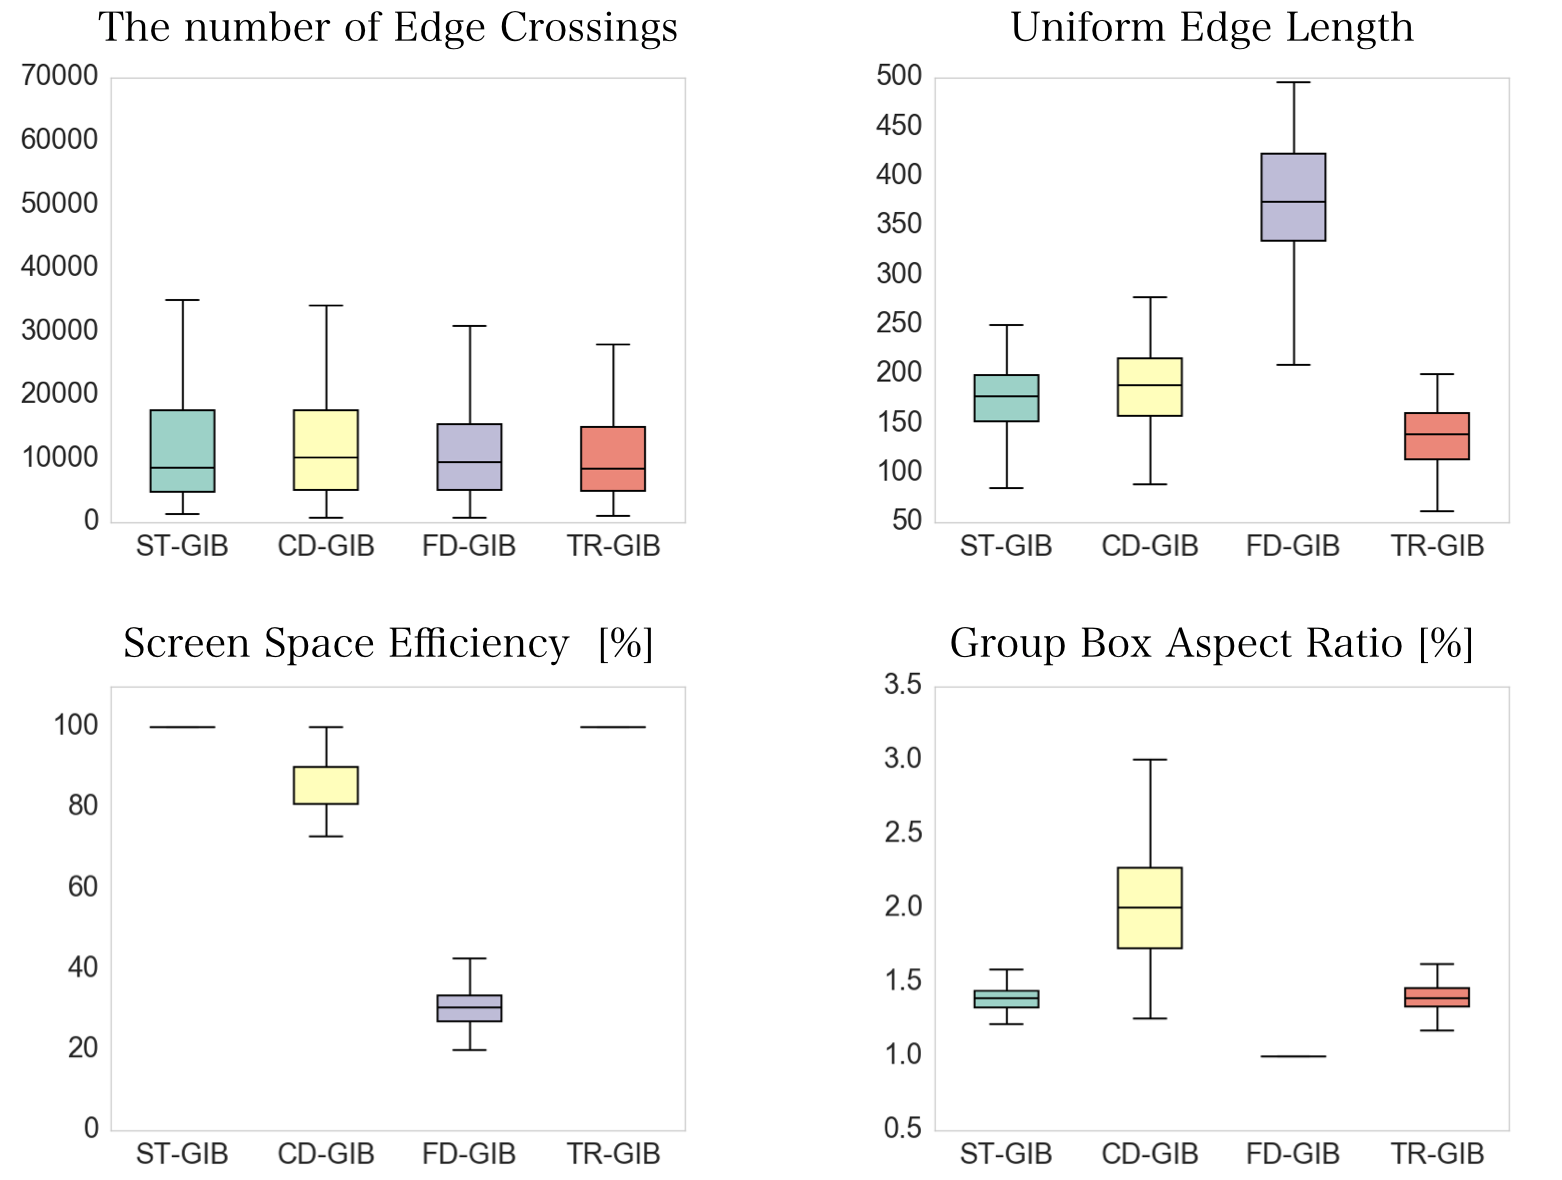
\includegraphics[width=15cm]{./images/4sta.png}
  \caption{実験1で用いたグラフにおける可読性に影響を与える指標の計算結果}
\end{figure}


\section{タスク}
\label{sec:task_ex1}
本実験におけるタスクはVehlowら\cite{Vehlow2017VisualizingGS}とSaketら\cite{saket2014group}の2つの調査論文を参考に決定した。
Vehlowらは複雑ネットワーク可視化手法の分類とともに、それらを評価するために用いられるタスクについても分類を行なっている。
分類にはGroup-only tasks (GOTs), group-vertex tasks (GVTs), group-edge tasks (GETs), group-network tasks (GNTs) の4種類が存在する。
GETはエッジがグループ化されているネットワークで使用可能なタスクのために、本実験にはこれを除いた3つのカテゴリのタスクが適用できる。
SaketらはGOTs, group-nodeタスク、group-linkタスク、GNTsの4分類でタスクを紹介している。
これら4カテゴリのタスクはすべて本研究に用いることが可能であるが、group-linkタスクはVehlowらの分類におけるGNTsに酷似している。
VehlowらとSaketらはそれぞれのタスク分類に対しタスクの例を紹介している。
我々はそれらの中から以下のタスクを選び用いた。
\begin{itemize}
  \item {\bf タスク1:グループタスク} ネットワーク内にいくつのグループが存在しているか。
  \item {\bf タスク2:グループ・ノードタスク} どのグループが一番大きい(小さい)か。
  \item {\bf タスク3:グループ・内部エッジタスク} どのグループが一番多く(少なく)内部エッジを含むか。
  \item {\bf タスク4:グループ・外部エッジタスク} どのグループが一番多く外部エッジを含むか。
\end{itemize}

タスク1はVeflowの分類におけるGOTsに属し、グループの数を判断するものである。
これはノードやエッジの情報を必要とせず、ネットワークグラフ全体を見ることが求められる。
このタスクによりネットワーク全体の構造を理解するのに適したレイアウトが明らかになると期待される。

タスク2はGVTsに属するもので、ノードの情報を理解することが求められる。
GIBにおいてはグループに含まれるノードの数は箱の大きさとして表現される。
グループの大きさは複雑ネットワークにおける重要な指標であり、これが読み取りやすいレイアウトほど良いとされる。
本タスクはグループの大きさが理解しやすいレイアウトを特定することを目指したものである。

タスク3はGNTsの一種であり、内部リンクに関するものである
内部リンクの可読性はネットワーク解析で重要な意味を持つ。
本タスクでは内部リンクの数の分かりやすさを通し、内部リンクの可読性を高めるレイアウトを明らかにすることを目指す。

タスク4もGNTsの一種であるが、タスク3と異なり外部リンクに焦点を当てたものである。
複雑ネットワークにおいては内部リンク同様外部リンクも重要な意味をもつ。
外部リンクの情報が理解しやすいレイアウトが本タスクで明らかになることが期待される。

タスク2とタスク3では被験者はノードおよびリンクが最大のグループと最小のグループを探す2種類のタスクに取り組む。
複雑ネットワークの解析では、グループはその大きさに関わらず理解しやすいことが求められる。
言い換えれば、大きいグループや小さいグループのどちらかのみが効果的に可視化されるレイアウトは実用的でない。
よってタスク2とタスク3では問題が半分終わった時点でタスクを変更した。
一方で、外部リンクが一番少ないグループを見つけることは非常に困難だったため、タスク4では外部リンクが一番多いグループを特定するという一種類のみを用いた。
問題があまりに難しい場合、被験者はランダムに解答してしまうために有意義なデータが記録できないと思われるからである。

\section{仮説}
\label{sec:hypothesis}
本節では実験で検証する仮説について記述する。
\ref{chap:GIBs}章で述べたように用いる4種のGIBは異なる特徴を持っているため、レイアウト毎にタスクの結果は異なると考える。
以下の仮説は各タスクにおけるレイアウトの効果と、その要因に関して述べたものである。
\begin{itemize}
  \item{\bf 仮説1} ST-GIBがタスク1で最も良い結果を残す。ST-GIBでは各箱が縦横に整然と並べられてる上その並びは箱の大きさの順であり、グループの数が数えやすいと考える。
  \item{\bf 仮説2} ST-GIBがタスク2で最も良い結果を残す。ST-GIBではグループはその大きさ順に並ぶため、一番大きい(小さい)グループは常に左上(右下)に配置される。被験者がレイアウトがST-GIBだと判別することができれば、答えを特定するのは容易だと思われる。
  \item{\bf 仮説3} CD-GIBはタスク2において他手法より有効でない。CD-GIBでは箱のアスペクト比が大きいためにその面積を視覚的に推定するのが難しく、良い結果を残せないと考える。
  \item{\bf 仮説4} TR-GIBはタスク3で最も良い結果を残す。TR-GIBはST-GIB同様にアスペクト比とスクリーン画面使用効率で優れているため、各グループがCD-GIBやFD-GIBよりも内部ネットワークが大きく描画される。
  加えてTR-GIBではエッジ交差数が少ないために内部エッジを外部エッジからの干渉なしに表現することが可能であると思われる。
  \item{\bf 仮説5} FD-GIBはタスク3において他手法より有効でない。FD-GIBでは箱が小さいために内部リンクが短くなり、リンクの数を把握することが難しいと考える。
  \item{\bf 仮説6} TR-GIBとFD-GIBがタスク4では有効と考える。TR-GIBはエッジ交差数が少なく、またFD-GIBはスクリーン使用効率こそ低いが外部リンクが描かれるための余白があるとも言える。
  これらのレイアウトは外部リンクの数を認識することが容易だと考える。
\end{itemize}

\section{実験デザイン}
本実験は、各タスクにおいてレイアウトのみ種類を独立変数とした多重比較検定を反復測定により行う。
グループの数などいくつかの値が刺激毎に異なるが、これらは正規分布に従っているため考慮しないものとする。

実験における各タスクはそれぞれのレイアウトが30問ずつの計120問で構成され、被験者は4タスクで計480問に取り組んだ。
被験者の慣れの影響を考慮し各刺激において異なるネットワークデータを用いた。
同じネットワークデータに4種類のレイアウトを適用し、タスクの結果を比較することも可能であるが、この場合被験者がレイアウトは異なるが同じデータを実験中に4回見てしまうために被験者がデータに慣れてしまうと考えたためである。
また実験中に視線データを記録する都合上、被験者は同じ順番で問題に取り組んだ。

刺激毎にタスクが異なると被験者が混乱するため、120問を完了するまで継続して一つのタスクを行なった。
各タスク内では問題の順番がランダム化されており、どのレイアウトが刺激として与えられるかはランダムとなっている。
同様に、疲労と慣れの効果を軽減するためタスクを行う順番は被験者毎にランダムにした。
各タスクは20問毎の6ブロックに分かれており、各ブロックが終わる毎に30秒ほどの休憩を挟んだ。
1タスクが終了すると5分までの比較的長い休憩を挟んだ。

\section{実験の流れ}
実験の前に、被験者に年齢、性別、勉強の分野などを問うアンケートを行なった。
その後生体計測や視線追跡、GIBレイアウトに関する説明を行った。
生体計測に関しては、被験者にその安全性やデータの取り扱いに理解をいただき同意書に署名を得た。
実験を行う前に、被験者がネットワークを理解し実験を行えるかを確かめるためにチュートリアルを行なった。
チュートリアルは本実験を模したものであり、データのみが本実験と異なっている。
被験者はチュートリアルを行うことで本実験前に各タスクに向けての準備を行った。

以上のプロセスの後本実験を行なった。
被験者はランダムな順番でタスクを行った。
タスク2とタスク3では\ref{sec:task_ex1}で述べたように60問毎に問題を切り替えた。
この際60問は4レイアウトが15問ずつで構成された。
タスクには時間制限を設けておらず、解答が行われるとサーバーに送信された。
被験者には解答時間よりも精度に重点を置くよう促した。
これは被験者が問題を早く解こうとすると誤答率が上がる他視線追跡データが実の無いものとなってしまい、本研究の意義にそぐわないためである。
図\ref{fig:screenshot_ex1}に実際の実験のスクリーンショットを示す。
これはタスク2において一番大きいグループを選ぶ問題であるが、グループがクリックされると選んだグループがハイライトされるようになっている。
エンターキーを押すと正否と完了時間が記録され、自動的に次の問題へと移行する。

本実験は人工照明で照らされた簡素な部屋で行われた。
実験に余計な干渉が入らないよう被験者は実験前に携帯電話の電源を切るように促された。
実験中、被験者は$1,920 \times 1,080$ピクセルのディスプレイから65cm離れた位置に顎台を持って顔を固定された。
視線追跡データはTobii Pro X3-1120により録画され、I-VTフィルター\cite{olsen2012tobii}を用いて眼球運動が注視か断続性運動かを判定した。

\begin{figure}
  \centering
  \label{fig:screenshot_ex1}
  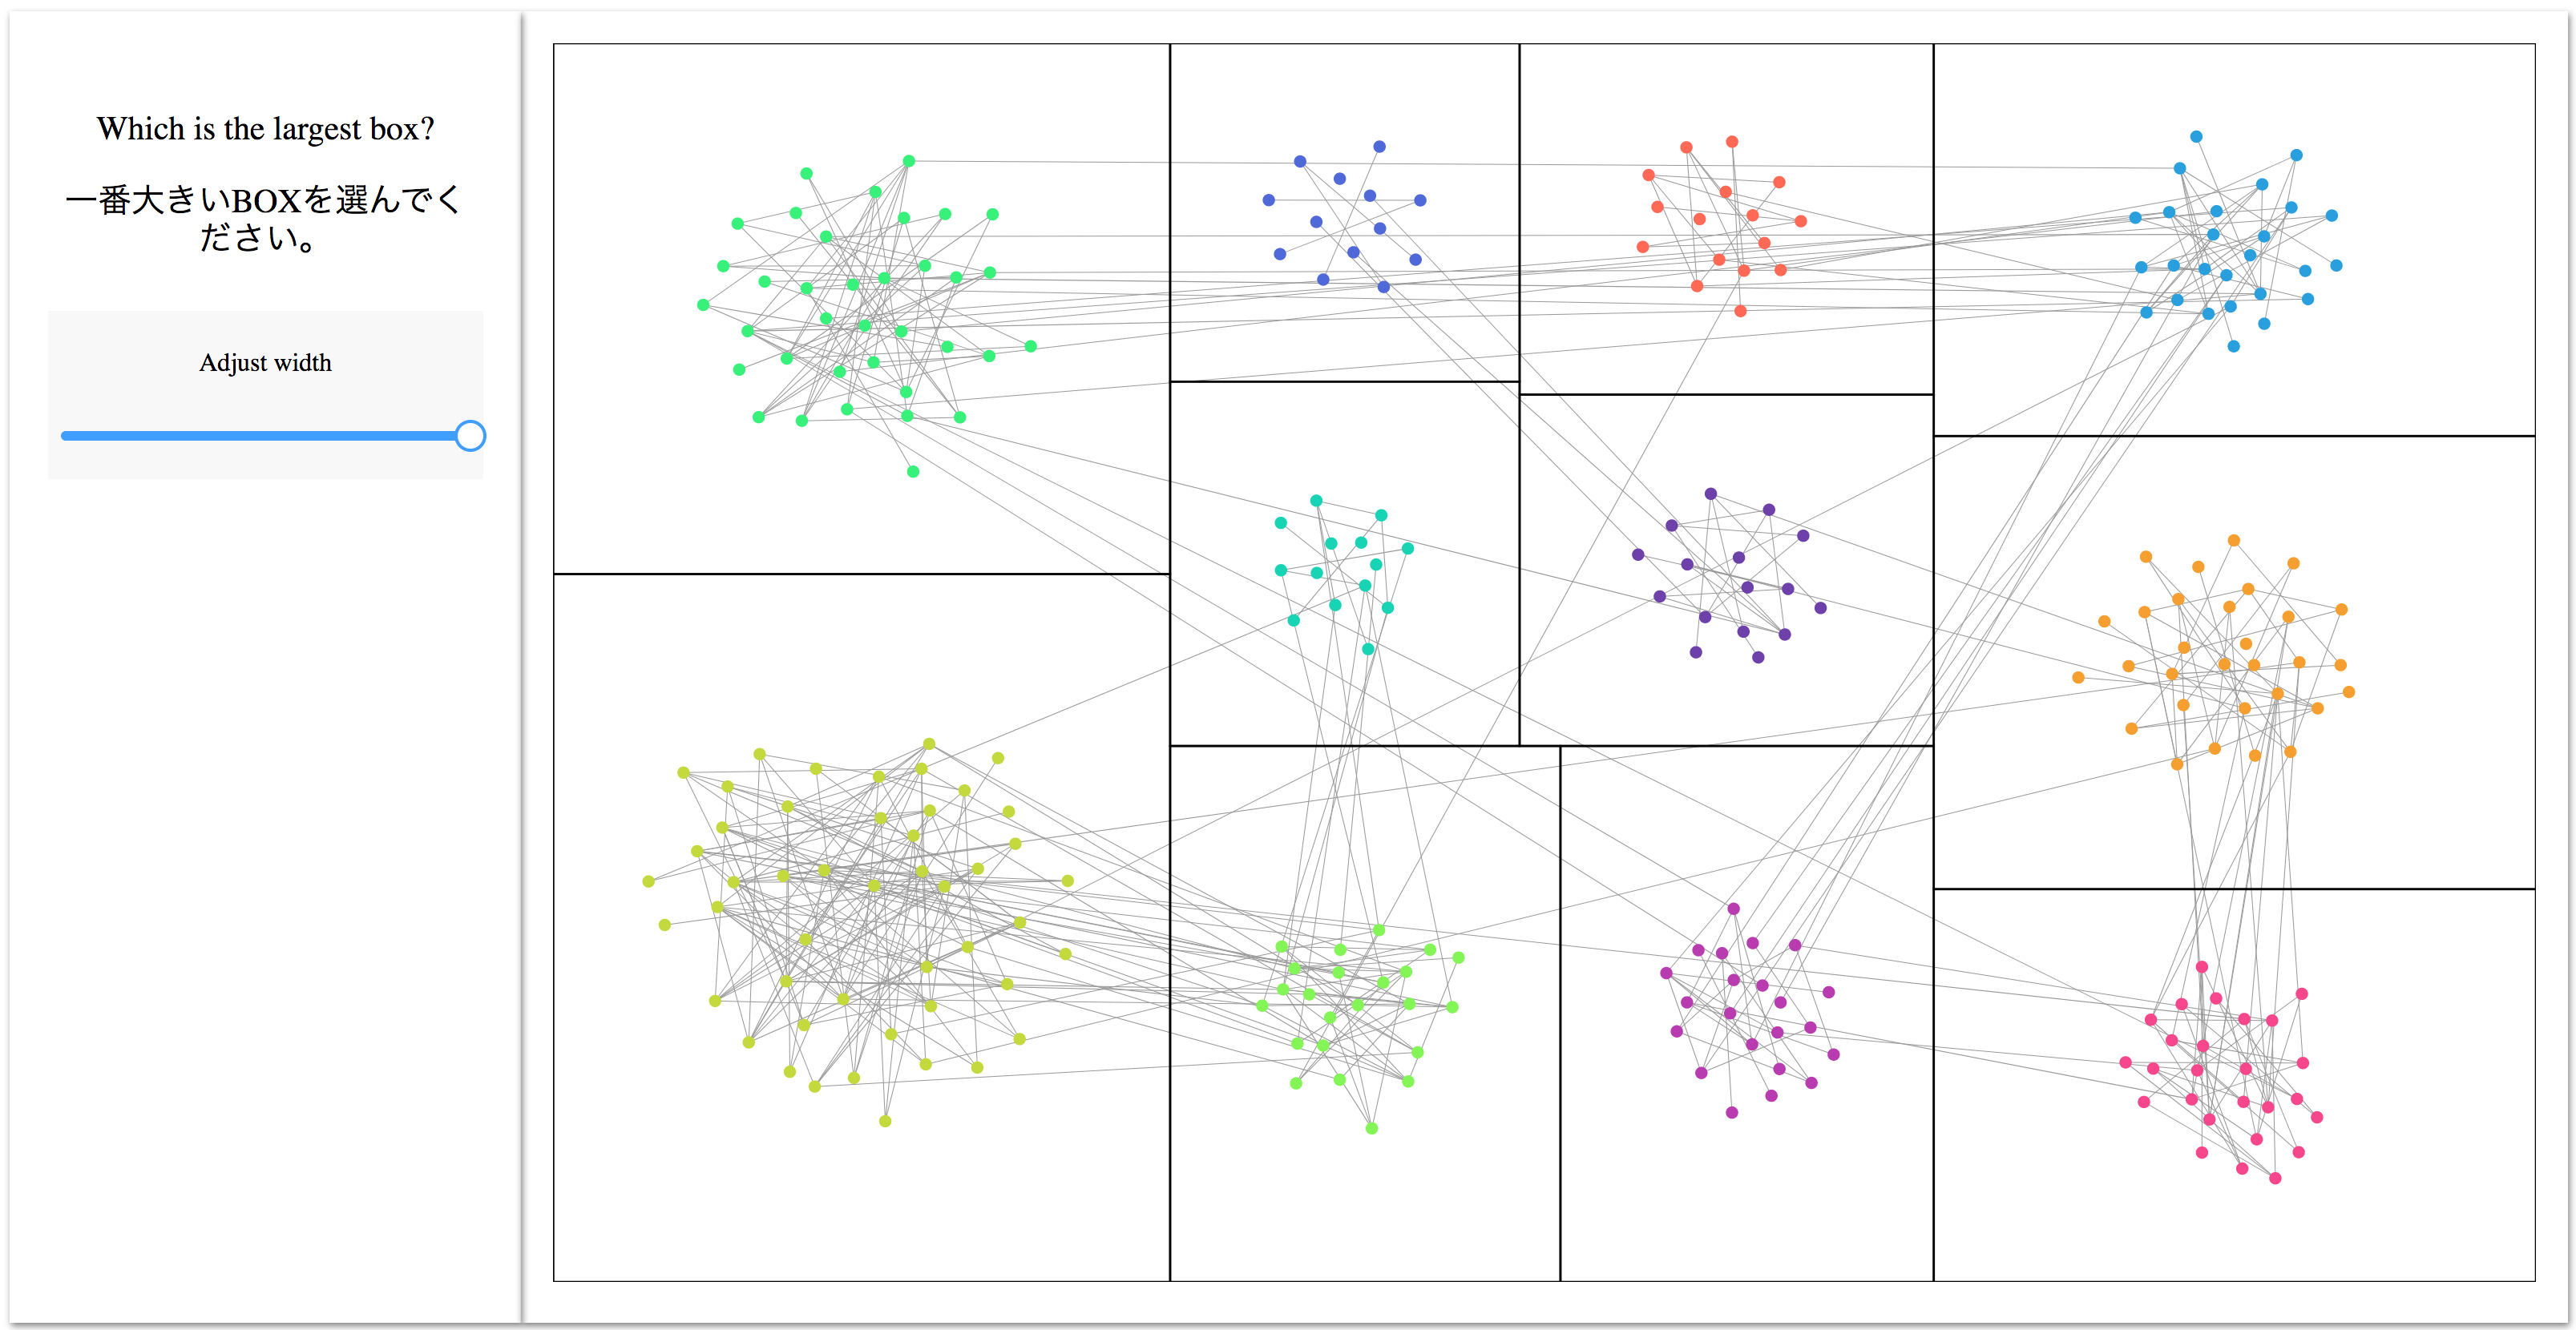
\includegraphics[width=15cm]{./images/screenshot.png}
  \caption{実験1のスクリーンショット。タスク2において一番大きいグループを選ぶ問題である。大きいグループをクリックしエンターを押すことで解答が送信される。}
\end{figure}

\section{被験者}
\label{sec:participants}
被験者は20人で、そのうち8人が女性、12人が男性であった。
このうち1名の被験者の実験中に技術的な問題が発生したため、計19人のデータのみを実験結果として用いる。
被験者の平均年齢は20.8歳で、最低年齢が18歳、最高年齢が24歳であった。
全員が日本国籍者かつ京都大学の学生であり、4人が工学を学んでいてその他は様々な分野の学生であった。
通常、日本では文章を左から右に読み、この方向はタスクに影響することが知られている\cite{yarbus1967eye}.
全被験者は正常もしくは矯正された視力を有していた。
実験は休憩を含み1.5時間から2時間ほど要し、被験者にはそれぞれ3,000円が支払われた。

\section{実験結果}
\label{sec:result_ex1}
本章ではユーザー実験の結果について記述する。
実験では正答率と完了時間に加え視線追跡データが測定された。
結果は2項に分けて述べる。
\ref{subsec:task_result_ex1}項ではタスクの正答率の完了時間について分散分析を行い結果を議論する。
\ref{subsec:eyetrack_result_ex1}項では視線追跡データに基づいて各仮説を検証する。

\subsection{正答率及び完了時間}
\label{subsec:task_result_ex1}
本項ではタスクにおける正答率及び完了時間をについて記述する。
データが正規分布に従っていなかったため、ノンパラメトリックな分散分析を行った。
Friedmanの検定を用いて4群間に有意差があるかを判定し、その後Wilcoxonの符号順位検定を行った。
全検定においてp値は0.05を用いた。
以下では各タスク毎の統計分析結果を述べる。
各レイアウトはその視覚的特徴の違いにより長所と短所があり、それゆえ全タスクは独立であると考えている。
図\ref{fig:result_ex1}に正答率と完了時間の結果を示す。

{\bf タスク1.} 全レイアウトでの平均正答率は97.7\%であり、平均完了時間は4480msであった。
Friedman検定により完了時間に有意差が確認され($p < 0.001$)、正答率には有意な差は見られなかった。
Wilcoxonの事後検定により、ST-GIBとTR-GIBでの完了速度ががCD-GIBとFD-GIBのものより有意に短いと明らかになった。
また、同様にCD-GIBとFD-GIB間にも有意差が見られ、CD-GIBの方が効果的であった。
被験者はST-GIBにおいてCD-GIBとTR-GIBにおいてよりも500msほど、FD-GIBにおいてよりも900msほど早くタスクを完了した。
これは仮説1を支持する結果となった。

{\bf タスク2.} ST-GIBは正答率が最も高いレイアウトであり、その正答率は89.6\%で完了時間が2425msであった。
完了時間はFD-GIBが最も短く、正答率は83.0\%で完了時間は2425msであった。
Friedman検定により、正答率と完了時間に有意差が見られた。
Wilcoxonの事後検定から、ST-GIBが他手法より正答率が高いこと(CD-GIBとFD-GIBに対し$p<0.001$、TR-GIBに対し$p=0.0041$)が分かり、またCD-GIBが他手法より正答率が低いこと(ST-GIBに対し$p<0.001$、FD-GIBに対し$p=0.0041$、TR-GIBに対し$p=0.0019$)が明らかになった。
これらの結果は仮説2, 3を支持するものであった。
FD-GIBとTR-GIBはCD-GIBより正答率が高かったが、グループがその大きさ順に並んでいるST-GIBには及ばなかった。

{\bf タスク3.} FD-GIBが正答率(78.8\%)、完了時間(3383ms)においても良い結果を時残した。
Friedman検定からこのどちらにも有意差が見られ、$p<0.001$だった。
Wilcoxon検定より、FD-GIBが他手法よりも正答率(ST-GIBとCD-GIBに対して$p<0.001$、TR-GIBに対して$p=0.017$)と完了時間(ST-GIBに対して$p=0.007$、CD-GIBとTR-GIBに対して$p<0.001$)の両方で有意な効果が見られた。
また、TR-GIBはST-GIB($p=0.039$)とCD-GIB($p=0.049$)より良い正答率を残した。
これらの結果は仮説4と5に反駁するものであった。
FD-GIBは正答率と完了時間の両面で最良の結果を残した。
TR-GIBはの成績は悪いものでは無かったが、正答率はFD-GIBより6\%低く、完了時間は500msほど長く要した。

{\bf タスク4.} 全体の平均正答率は61.2\%、平均完了時間は5405msであり、Friedman検定により完了時間($p=0.039$)のみに有意差が見られた。
Wilcoxonの事後検定によりTR-GIBの完了時間がFD-GIBのものより有意に短いことが観察され、仮説6を裏付ける結果とはならなかった。


\begin{figure}
  \centering
  \label{fig:result_ex1}
  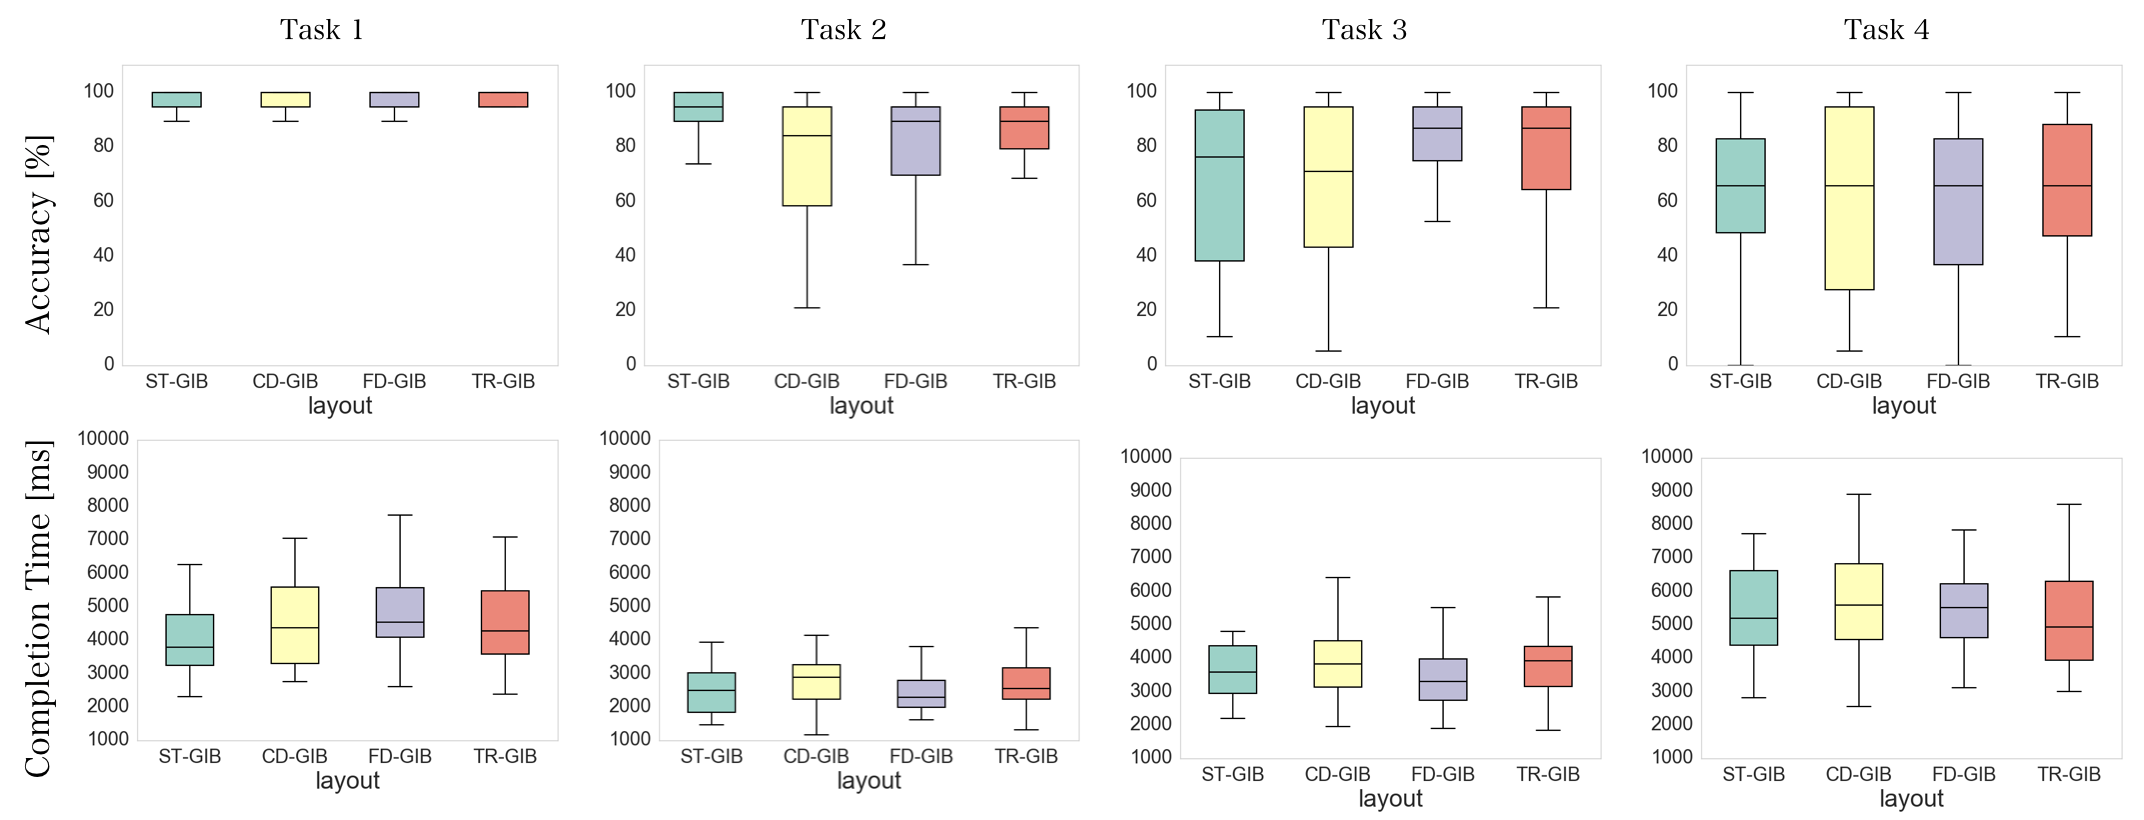
\includegraphics[width=15cm]{./images/8sta.png}
  \caption{実験1のタスク結果を箱ひげ図で表したもの。上段はタスクの正答率、下段は完了時間を示す。}
\end{figure}

\subsection{仮説検証}
\label{subsec:eyetrack_result_ex1}
本項では視線追跡データに基づき各仮説について議論する。
視線追跡データの解析には主に2種類の方法がある。
一つ目は注視点座標や注視時間などの定量化できる指標を用いて統計的に議論するもの、二つ目はAOIや注視点の軌跡に基づき視覚的に解析を行うものである。
定量的な指標として、本実験では{\bf DB}と{\bf DA}という指標を計算している。
これらは被験者が正解のグループ以外のグループを注視した数に関するものである。
被験者が初めて正解のグループを注視するまでにそれ以外のグループを注視した回数をDB (Distractors Before target)、被験者が初めて正解のグループを注視してからそれ以外のグループを注視した回数をDA (Distractors After target)としている。

視覚分析は視線データを軌跡マップやヒートマップとして可視化し解析するものである。
Burchらは視線追跡データの視覚分析手法をその特徴ごとに消化している。\cite{Burch2013VisualTS}
我々はBurchらの手法を参考に、データ解析に用いる視覚分析手法を厳選した。
図\ref{fig:AOI-based-analisys}は各タスク、各レイアウトのある刺激に対し、2種類の可視化手法で注視するAOIの時間変動性を示したものである。
左側の図はそれぞれの被験者がタスクが終了するまでにどのAOIを見ていたかを表すものである。
この図では被験者は上からタスク精度が高く完了時間が短い順に並んでいる。
右側の図はタスク完了までにそれぞれのAOIを注視していた人数を表したものであり、最も上の被験者はタスクを正確にかつ最短時間で完了している。
両図ではデータの前処理として、刺激毎に被験者のタスク開始時間と終了時間を揃え、タスクに要した時間を線形に1,000のセグメントに分割している。
図\ref{fig:AOI-based-analisys}の左側の図より、被験者が各刺激でAOIを見る順番が似ていることが分かった。
これはタスクを完了する時間に関わらずタスクを解く戦略が似ていたこと{}を示唆しており、またこの傾向は特にタスク2とタスク3で顕著であった。
本実験で視線追跡データを計測する目的はタスク結果に影響する要因を特定するためである。
それゆえ、以降は\ref{sec:hypothesis}節の仮説に基づき、タスク結果に寄与する視覚的要素に焦点を置き議論する。

{\bf 仮説1.} 本仮説はタスク1においてST-GIBが最も有効であったため実証された。
仮説検証のため、タスク完了に要した注視店の数を計算し、その結果を\ref{table:gazecount-task12}に示す。
ST-GIBは他手法よりも注視回数が少なく、これは被験者がグループの数え直しが少なく、また一度の注視により複数のグループを数えることができたことを示唆している。
また、図\ref{fig:AOI-based-analisys}の左側の図より、ST-GIBとTR-GIBでは被験者がグループを同じ順番で注視していることがわかる。
これは全ての被験者が同様の戦略でタスクを解いていたことを意味する。
図\ref{fig:AOI-based-analisys} (a)の右の図より、被験者は左上のグループから右下に向かい数を数えていったことがわかる。
これは主に日本人が文章を左から右に、上から下に読むことに起因すると思われる。

以上から、ST-GIBの有効性は被験者がとる戦略の頑強性と一度に複数のグループを数えられることによるものだと考えられる。
CD-GIBやFD-GIBでは箱が縦横に均一に並ばないために、被験者は刺激毎に異なった順番で箱を数える必要がある。
しかし、常に同じ順番で数えることができないと、既に数えた箱を忘れてしまい、数え直しを行いタスク完了に時間がかかることもある。
また、縦横方向に箱が整然と並んでいるために隣り合う箱を同時に数えることも容易である。
以上の理由は箱が縦横方向に整然と並ぶ、ST-GIBのグループ整然性によるものだと考える。

{\bf 仮説2.} タスク2の結果より、ST-GIBが最も有効であるという仮説2が支持された。
表\ref{table:gazecount-task12}から、CD-GIBとTR-GIBに比べ、ST-GIBとFD-GIBではタスクに要した注視回数が少ないことがわかる。
また、表\ref{table:db_and_da_task12}に示す通り、ST-GIBでは{\bf DB}が他手法よりも小さかった。
これは被験者が正解のグループに早くたどり着いたことを示す。
タスク2でとられた主な戦略は、大きいグループをいくつか選び、それらを見比べて解答を選ぶというものであった。
{\bf DB}は大きいグループを抽出する第一プロセスでのレイアウトの有効性に言及し、{\bf DA}は候補を見比べ大きさを比較する第二プロセスに関するものであると言える。

ST-GIBではグループがその大きさの順で並んでいるために、これが影響し第一プロセスでの難易度が低かったのだと考える。
また、図\ref{fig:AOI-based-analisys} (b)はST-GIBが第二プロセスでも有効であったと示唆している。
タスク完了の直前で注視されたグループは大きさ比較の候補であると考えられるが、ST-GIBではこれらの箱が近くに配置されている。
ST-GIBは両プロセスにおいて有効だったために良い結果が出たと考える。

{\bf 仮説3.} タスク2においてCD-GIBが他手法よりも正答率が低かったため、この仮説は支持された。
これはCD-GIBにおける箱のアスペクト比が悪いために、グループの大きさを比較するのが難しかったことが原因と考える。
また図\ref{fig:AOI-based-analisys} (b)から結果に影響する他の要因が示唆されている。
CD-GIBにおいて、視線が集中していた2つのグループが他のレイアウトよりも遠くに配置されていた。
CD-GIBでは大きさが似ている箱同士が離れて配置されることがあり、これが大きさの比較を困難にした。
以上二つの理由により、CD-GIBはタスク2で良い成績を残せなかったと考える。

{\bf 仮説4.} タスク3ではTR-GIBよりもFD-GIBの方が好成績を残し、仮説3は実証されなかったが他の2手法よりは良い結果となった。
図\ref{fig:AOI-based-analisys} (c)によると、本タスクでの被験者の主な戦略はグループの大きさを見るというものであった。
本タスクは内部リンクが多い(少ない)グループを探すというものであったが、データ生成のアルゴリズム状大きなグループは内部リンクが多く、小さいグループは内部リンクが少ない傾向にある。
そのため被験者はまずグループの大きさを見ていくつか候補となるグループを抽出し(第一プロセス)、その後それらのグループを相互に見て比較をした(第二プロセス)のだと考える。

タスク2と同様、{\bf DB}と{\bf DA}がそれぞれ第一、第二プロセスの難易度を示すと考え、これらは表\ref{table:db_and_da_task3}に示される。
ST-GIBとTR-GIBは{\bf DB}が少なく、これらのレイアウトは箱の大きさを比べるタスク2においても良い成績を残したために第一プロセスにおいて有効であったと言える。
一方で図\ref{fig:AOI-based-analisys} (c)より、第二プロセスを表すタスクの後半においてST-GIBは注視点が散在しているのに対しTR-GIBでは内部リンクが多いグループに注視が集中していることが分かる。
しかし、{\bf DA}はTR-GIBの方がST-GIBとCD-GIBよりも多かった。
我々はこれがST-GIBとCD-GIBにおいて第二プロセスにおける比較作業が有意義でなく、被験者が誤った答えに早くたどり着いたのだと思われる。
ST-GIBとCD-GIBはタスク3で誤解を招きやすく、それゆえ{\bf DA}が他手法より小さかったと考える。
TR-GIBの第二プロセスで有意義な比較作業が行えたのはエッジ交差数の少なさによるものであろう。
内部リンクが外部リンクの干渉を受けることなく描画されるために、内部リンクの数を正確に視認でき、精緻な比較作業が行われたと考える。

{\bf 仮説5.} タスク3においてはFD-GIBが最も効果的であり、仮説5に反駁する結果となった。
FD-GIBの{\bf DB}は比較的大きかったため、第一プロセスにおいては他手法に比べ有効では無く、その有効性は第二プロセスにより確立されたと考える。
FD-GIBにおける{\bf DA}が他手法より少なかったことから、これは支持され、FD-GIBでは内部リンクの数を視覚的に判断することが容易であったと思われる。
我々はこれがエッジ交差数が少なかったことと、FD-GIBにおいて各グループが小さく描写されることに起因すると考える。
TR-GIB同様FD-GIBではエッジの交差数が少なく、正答率を高めた。
また、本実験においてはエッジが灰色に描かれたため、その密度がエッジの濃淡として表され、グループ内部の色を判別することが内部リンクの数の認識につながった。
FD-GIBは箱が小さいためにこの傾向が強く、そのため被験者は内部エッジの数を視覚的に容易に計ることができたと考える。

{\bf 仮説6.} タスク4ではTR-GIBがFD-GIBより完了時間が短かったが、正答率に有意な差は見られなかったため仮説6は実証されなかった。
図\ref{fig:AOI-based-analisys} (d) から、殆どのレイアウトにおいて注視点が多くのAOIに散在していること一方で、CD-GIBでは中心のグループがよく注視されていることが分かる。
CD-GIBにおいては、それが正解であるかどうかに関わらず中心の箱が頻繁に注視されていた。
このグループが繋がっているグループの数が最も多いために、外部リンクがこの箱の周辺に描画されることが多いのである。

ここから、被験者は本タスクにおいて外部リンクの束を手掛かりにタスクに取り組んでいたことが分かる。
CD-GIB以外のレイアウトで注視点が散在していたのも、外部リンクが様々なAOIに跨り存在しているからだと考えられる。
本実験で用いたデータでは。いくつかのグループのペアが強い接続を持つために、外部リンクの束が生まれる。
図\ref{fig:concentration}に本タスクのある刺激における被験者の視線軌跡マップを示す。
この図ではピンクの線で表される視線の動きが外部リンクの束に重なっており、ここからも被験者が外部リンクの束を手掛かりにタスクを解いていたことが分かる。

正答率に差が出なかったのは、平均正答率が61.2\%とタスクが難かしかったこととも影響すると思われる。
タスクの難易度が高い場合、被験者が解答を乱雑に選びレイアウト間に差が出なくなることも考えられる。
また、リンクの束を認識するという意味においては、従来可読性を高めると考えられるエッジ長の均一性や外部リンクを短くし交差数を減らすこともあまり有意義ではないとも考えられる。
長いエッジの束は特定しやすくいが、短いエッジの束はスクリーンにおける占有面積が少ないために判別しづらく、タスクに予期しない効果をもたらしたとも考えられる。

\begin{figure}
  \begin{center}
    \label{fig:AOI-based-analisys}
    \includegraphics[width=14cm]{./images/long.pdf}
    \caption{視線追跡データの時間変動制を可視化するAOIベースの視覚解析図。各タスク、各レイアウトに対し2種類の手法の可視化図を表示している。左の図は全被験者が解答までに注視したAOIを順に表している。この図では、被験者はタスク精度と完了時間の順に上から並んでいる。右の図はAOIを注視している人数の時間変動を示したものである。}
  \end{center}
\end{figure}

\begin{table}[b]
  \begin{center}
  \caption{タスク2における{\bf DB}と{\bf DA}の平均 (標準偏差).}
  \label{table:gazecount-task12}
  \begin{tabular}{|c|c|c|c|c|} \hline
  & ST-GIB & CD-GIB & FD-GIB & TR-GIB \\ \hline
  % Task 1 & 12.5 (5.49) & 14.4 (6.79) & 15.6 (6.85) & 14.1 (6.31) \\ \hline
  {\bf DB} & 3.6 (3.59) & 3.9 (3.67) & 4.1 (3.48) & 3.7 (3.06) \\ \hline
  {\bf DA} & 2.84 (3.33) & 2.99 (3.67) & 4.1 (3.48) & 3.7 (3.06) \\ \hline
  \end{tabular}
  \end{center}
\end{table}

\begin{table}[b]
  \begin{center}
  \caption{タスク3における{\bf DB}と{\bf DA}の平均 (標準偏差).}
  \label{table:db_and_da_task3}
  \begin{tabular}{|c|c|c|c|c|} \hline
  & ST-GIB & CD-GIB & FD-GIB & TR-GIB \\ \hline
  % Task 1 & 12.5 (5.49) & 14.4 (6.79) & 15.6 (6.85) & 14.1 (6.31) \\ \hline
  {\bf DB} & 3.8 (4.64) & 5.1 (5.11) & 4.8 (4.38) & 3.8 (4.48) \\ \hline
  {\bf DA} & 4.8 (4.65) & 4.8 (4.84) & 3.7 (4.27) & 5.3 (5.37) \\ \hline
  \end{tabular}
  \end{center}
\end{table}

\begin{figure}[t]
  \begin{center}
  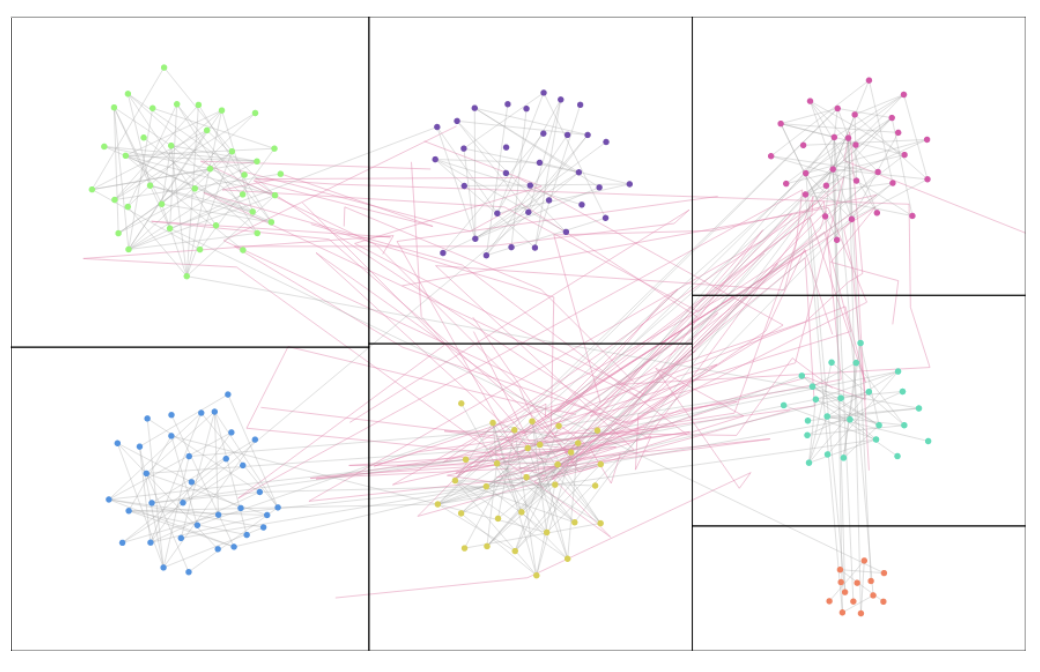
\includegraphics[width=15cm]{./images/concentration.png}
  \caption{タスク4における視線の軌跡マップ。視線の動きはピンクの線で表され、外部リンクの束と重なって動いていることが分かる。}
  \label{fig:concentration}
  \end{center}
\end{figure}

\section{考察}
視線追跡システムを用いた実験により、GIBについて興味深い事実がいくつか見つかった。
本節では各タスクに分けてそれらを記述する。

{\bf タスク1.} グループの数を数えるというシンプルなタスクであったが、その完了時間には有意な差が見られた。図\ref{fig:AOI-based-analisys} (a)から、ST-GIBが有効性はそのグループの整然性によるものだと示唆された。
グループがスクリーン内に散在するFD-GIBでは完了時間が最も長かったことからもこれは支持される。
グループの整然性から、被験者は頑強な戦略と一度に複数のグループを数える効率的な行動がとれた。

{\bf タスク2.} グループの整然性とアスペクト比が1に近いST-GIBが最も良い成績を修めた。
グループが正方形に保たれるFD-GIBが高い正答率と最も短い完了時間を持ち、アスペクト比が悪いCD-GIBは最も正答率が低かった。
これらの結果から、先行研究で報告されている通り\cite{shneiderman1992tree}アスペクト比が箱の大きさを推定するのに大きく影響することが確認された。

また、視線追跡データを解析することで本タスクに影響する他の要因を特定できた。
図\ref{fig:AOI-based-analisys} (b)より、CD-GIBでは大きさの比較が行われたグループが離れて配置されていることが分かる。
ST-GIBやTR-GIBのような大きさの似たグループが近くに配置されるグループでは被験者は好成績を残したことから、比較対象となるグループ間の距離が重要であることが分かった。

これはグループの大きさを見分けるタスクのみならず、様々なタスクでも重要な意味を持つ要因である。
表現型ネットワークにおいても、複数の注目するノードを比較するといったタスクは実際に行われる。
こうした際に、ノードの属するグループが異なる場合は、それらのグループが近くに配置される必要がある。
これは可視化のインタラクティブ性にも言及する点である。
箱の位置を任意に動かすことができれば、比較するグループを近くに配置することができる。
特にFD-GIBでは箱を他手法よりも自由に動かすことができ、利点は大きいと思われる。
ST-GIBやTR-GIBでもグループの並び替えることができるため、そうしたインタラクションが実装されれば効率は上がると考えられる。

{\bf タスク3.} このタスクでは被験者は内部リンクの数を判別することが要求された。
我々はエッジ交差数を減らすことがこのタスクにおいて重要だと考えていた。
エッジ交差数の少ないTR-GIBとFD-GIBでは、期待通り高い正答率が得られた。
先行研究と同様に、エッジ交差数を減らすことの重要性を裏付ける結果となった。

視線データの計算的手法である{\bf DB}と{\bf DA}や図\ref{fig:AOI-based-analisys}に示される視覚分析もこれを支持している。
本タスクにおいて被験者はまず第一プロセスとして解答の候補となるグループを抽出するためグループの大きさに注目し、その後第二プロセスとして候補のグループを比較したことが分かった。
TR-GIBは{\bf DB}が小さく第一プロセスで効果的で、第二プロセスでは{\bf DA}が大きく解凍に時間はかかったが有意義な比較が行われ、高い正答率につながった。
高い正答率を持ちながら比較の回数が多いのは、ST-GIBやCD-GIBでは内部エッジが外部エッジに覆われ解答をミスリードしていた一方、TR-GIBでは内部エッジの視認が容易で比較作業が精緻に行えたからであると考える。
FD-GIBは正答率が最も高く{\bf DA}が最も小さかった。
これは被験者が最初に正解であるグループを見てから、解答を完了するまでに他のグループと比較をする回数が少なかったことを示している。
これは被験者が内部リンクの数をエッジの密度により生まれる色の濃淡として知覚し、特に各グループが小さく描画されるFD-GIBではこの傾向が強くなっただと考えられる。
先行研究に反し、本タスクにおいては箱の面積が小さい方がユーザーのタスクパフォーマンスが向上したと考えられる。

この点は非常に興味深い点である。
本タスクはどのレイアウトが最も内部リンクを表現するのに適したレイアウトかを明らかにすることを目的としたものであったが、実際は被験者はグループ内部の色の濃淡など我々の期待よりも抽象的な情報を探すタスクとなってしまった。
しかし、抽象的な情報を要するタスクにおいては箱は小さい方が有効であると判明した。

複雑ネットワーク解析では、抽象的な情報と具体的な情報を交互に見ることが度々求められる。
このうち抽象的な情報を見るには、各グループを小さに描写し、全体のトポロジーを優先したグラフの方が効果的と示唆された。
一方で、各ノードのつながりなどを具体的に論じるにはグループを大きく描写する必要性がある。
特に、グループ間をまたがるエッジについて議論したい場合はFD-GIBのようにグループ同士が離れて描写されるレイアウトでは可読性が制限される。
上述したように、FD-GIBはその自由度からインタラクションに向いたレイアウトであるが、インタラクティブにグループの座標を変更することはエッジ交差数を増加させ可読性を減少させてしまうこともある。
より具体的で詳細な情報の認識にどのレイアウトが有効であるかはさらなる議論が必要である。

{\bf タスク4.} 本タスクでは正答率に差が確認されなかった。
この原因には様々なことが考えられるが、外部リンクの可読性に関して4手法間に差は見られなかった。

{\bf 概括} 各レイアウトはタスクによりトレードオフがあることが確認された。
また、平均の正答率の差が小さい場合でも分散や最小値には大きな差が見られることがあった。
例えば、タスク3でのFD-GIBの正答率がTR-GIBよりも6\%ほど高いのみだったが、最低値にはかなりの差が見られた。
ST-GIBはタスク1, 2で最良の結果を残した一方、CD-GIBは全タスクを通して効果的で無かった。
FD-GIBはタスク3で最も良い結果を残した他、タスク2でも有効であった。
TR-GIBは全タスクを通してその有効性を示した。

ST-GIBはタスク1, 2においては最も良い結果を残したが、内部エッジを表現する点においては他手法より劣った。
複雑ネットワークの解析において内部エッジの効果的な表現は不可欠であり、この点においてFD-GIBとTR-GIBの方が優れたレイアウトであると考える。
現実の複雑ネットワークでの解析作業を考慮すると、タスク1, 2で優秀な成績を残し、かつタスク3でST-GIBを上回ったこれら二つのレイアウトが最も効果的であると考える。

しかし、タスク3で確認したようにこれらにはトレードオフがあると思われる。
FD-GIBは内部リンクの多さといった抽象的な情報の表現ではTR-GIBより効果的である。
しかし箱が小さいためにノード同士の繋がりといった具体的な情報の表現ではTR-GIBの方が有効であるとも考えられ、これらを併用することで効率的な解析作業が行えるかもしれない。

また、本実験では使用したデータに含まれるノードとグループの数が正規分布により決められた。
これによりより一般性を持たせた場合での各レイアウトの有効性を議論したが、近年では可視化手法のデータ拡張性についての研究が進んでいる。
特に、膨大なネットワークではそのコミュニティを検出する重要さが知られており、複雑ネットワークを構成する。
今回用いたデータでは平均のノード数が240とそこまで多くはない。
データが大きい際に各レイアウトがどのような効果をもたらすかは本実験で未解明な部分である。

\chapter{実験2}
\label{chap:ex_2}

実験1ではST-GIB、CD-GIB, FD-GIB, TR-GIBを対象とした4タスクからなるユーザー実験により、FD-GIBとTR-GIBの優位性が明らかになった他、これら二つのレイアウトにトレードオフがあることが示唆された。
FD-GIBは抽象的な情報を表示する旨では有効であるが、各グループが小さく描画されるためにより詳細な情報を求められるタスクにおいてはTR-GIBの方が効果的かもしれない。

また実験1の限界として、各レイアウトのデータ拡張性に言及していないという点が挙げられた。
実験1よりも多くのノード、グループが存在する時に各レイアウトの有効性がどう変化するかは未だ未解明であり、表現系ネットワークの可視化においても重要な意味を持つ。
現在理化学研究所において用いられている表現型ネットワークのデータは8細胞期までの22グループを持つものと、64細胞期までの77グループを持つものの2種類がある。
C. elegansの表現型データの計測精度はバイオイメージ・インフォマティクス技術や生物学研究者たちの用いる手法によるところが大きく、今後も異なる大きさのデータを用いて解析を行うと考えられる。
複雑ネットワークを可視化するGIBは様々な量のデータを効果的に可視化することが求められるため、そのデータ拡張性が明らかになることによりネットワーク解析の効率も向上するであろう。

以上二つの理由から、我々は一つ目の実験で未解明だった部分を明らかにするため、二つ目の実験を行う。
実験2では、実験1で有効であったFD-GIBとTR-GIBを対象に、実験1よりも大きなデータを用い、実践的で複雑なプロセスを要するタスクを行う。
また実験1と同様に実験中は視線追跡データを記録した。
本章では実験2の目的、方法、結果について詳細に述べる。

\section{タスク}
\label{sec:task-ex2}

実験2では、その他の要素に先立ちタスクについて記述する。
以降に述べるデータ生成や実験デザインは本項で定めるタスクに基づき決定されたものである。

本実験は実験1よりも詳細な情報、作業を要する複雑なタスクを用いてFD-GIBとTR-GIBの差を確認することを目指す。
そのため目的に適したタスクを入念に選ぶ必要がある。
Vehlowら\cite{Vehlow2017VisualizingGS}とSaketら\cite{saket2014group}の紹介したタスクの中で、この目的に沿うものを以下に列挙する。
\begin{enumerate}
  \item 与えられた複数のグループを繋ぐ最短パスを探す
  \item 異なるグループに属する2ノードを繋ぐ最短パスを探す
  \item 異なるグループに属する2ノードを繋ぐ最短パスが必ず訪れるグループの数の最小値を探す
  \item 最も次数の高いノードを含むグループを探す
\end{enumerate}
これらはグループ間を跨いだ解析が必要な他、あるノードに着目しそれに繋がるノードを探すといった詳細な視点も必要とされるため、本実験の目的に合致すると思われる。

この中から我々は{\bf 2. 異なるグループに属する2ノードを繋ぐ最短パスを探す}タスクを選択した。
大規模なネットワークでは最短パスが複数生まれるため、3.の答えは幅広くなってしまい、また数を答えるタスクは被験者が乱雑に答えてしまうおそれがある。
4. はグループやノードが多いと難易度が期待よりも高くなってしまう。
1.と2.はどちらも本実験に適したタスクだと考えたが、問題の難易度や実装面での可用性を考慮し2.を用いることとした。

本タスクではまずネットワーク内の異なるグループに属する2ノードが与えられ、最短パス構成する全ノードをクリックすれば正解となるものとする。
こうしたタスクにおいては実験におけるインタラクションの設計が大きな影響を与えると知られている\cite{yoghourdjian2018exploring}.
ノードをクリックした際の反応を変えると、タスクの難易度やそれに含まれるサブタスクが変わり、実験により議論できる点が変わってくる。

本実験では以下のようなインタラクションを実装した。
\begin{itemize}
  \item はじめに与えられるノードは赤く色付けされ、他のノードは黒色である。
  \item エッジは灰色であり、重なりを表現するため半透明である。
  \item クリックされているノードは各々異なる色で色付けされる。
  \item クリックされているノードやマウスオーバーされているノードは他のノードより大きく描かれる。
  \item クリックされているノードに接続されるエッジはノードと同じ色で色付けされる。
  \item はじめに与えられるノードは既にクリックされた状態で問題が始まり、接続されるエッジは青い色で色付けされる。
  \item クリックされているノード同士を繋ぐノードは赤い色で色付けされる。
  \item 正解のパスを構成するノードを全て選ぶと、パス全体がピンクに色付けされ、次の問題へ移行する。
\end{itemize}
以上のインタラクションが実装された実験画面の例を図\ref{fig:screenshot-ex2}に示す。
赤いノードからは青いエッジが、クリックされている緑と黄色のノードからはノードと同じ色のエッジが生えている。
ノードやエッジに色付けなどを行うのはユーザーの解答を補佐するためであり、難易度を下げるためにこれらのインタラクションを用意した。
これらのインタラクションではグループ間を跨いでここのノードの繋がりに着目するという本来の目的を阻害することがないと考える。
ネットワーク解析ツールではノードにマウスオーバーすると関係するエッジがハイライトされるというインタラクションが用いられるが、これは本実験では用いない。
というのも、被験者がランダムにノードにマウスを合わせ、繋がりの有無を見ることが予想されるからである。
ネットワークの構造やノード間を注視し、必要最低限のインタラクションで解答を行わせるために、過度な修飾は避けた。

また、以上の設定のみではタスクが困難でデータに乱雑性が生まれるため、以下の設定を行い難易度や実験条件をを調整した。
\begin{enumerate}
  \item 最短パスを構成するノード数は5である。
  \item 7ノードまでのパスは正解とする。
  \item 正解のパスは複数あり、最短パスも複数存在しうる。
  \item はじめに与えられるノードからは必ず二本以上のエッジが生えている。
  \item 最短パスに含まれるノートの中で、同じグループに含まれるものは最大で2つである。
\end{enumerate}
1.から3.は難易度を調整するために設定したものである。
赤いノードに繋がるエッジが一本しかない場合、パスに含まれるノードが自動的に一つ決まり、最短パスの構成ノード数が4となり実験条件が異なってしまうため4.を設定した。
5.はタスクの内容を統一し、刺激により難易度を変えずにかつ実験結果に均質性を持たせるための設定である。
最短パスのうち4ノードが同じグループに含まれる刺激と、多数のグループを経由する刺激では被験者が行う作業が異なってくる。
一問を完了するのに数十秒を要する複雑なタスクでは、被験者のとる戦略によりいくつかの部分タスクに分割される。
今回のタスクでは、赤いノードを探す、繋がりそうなパスの方向を決定する、ノードのつながりを詳細に見てノードを繋ぐといった部分タスクが考えられる。
各刺激によって各部分タスクが占める割合が異なると、解析が困難になる。
我々は5.の条件を付加することで部分タスクの割合を刺激感で均質にすることを目指した。
また、この条件により被験者はグループ間の繋がりを積極的に見る必要が生まれ、この効果も内部リンクと同様に外部リンクの表現にも重点を置くGIBの評価には有効である。

しかし、以上の条件は被験者にも説明されたため、これらは被験者の行動を左右しうる。
特に5.の条件により、我々は被験者はタスクのはじめに経由するグループを探すはずと考えた。
これはパスを繋ぐという本来のタスクの意味からは離れたものであり、我々の意図したものではない。
最短以外、つまり6, 7ノードを経由するパスであれば、2ノードが属する2グループのノードのみでパスを構成できるため、これも被験者には説明したが、被験者の行動を制御できたわけではない。
しかし、部分タスクを制御できかつ内部リンクと同様に外部リンクも被験者に意識づけさせることができるこの条件の利点は、欠点よりも大きいと考えた。

以上のタスクを構成することにより、我々は2手法の内部リンクと外部リンクの表現に関する有効性を確かめられると考えた。
また、様々なインタラクションや条件を持ってタスクを制御することにより、得られるデータの均質化と信頼性の向上を図った。

\begin{figure}[t]
  \begin{center}
  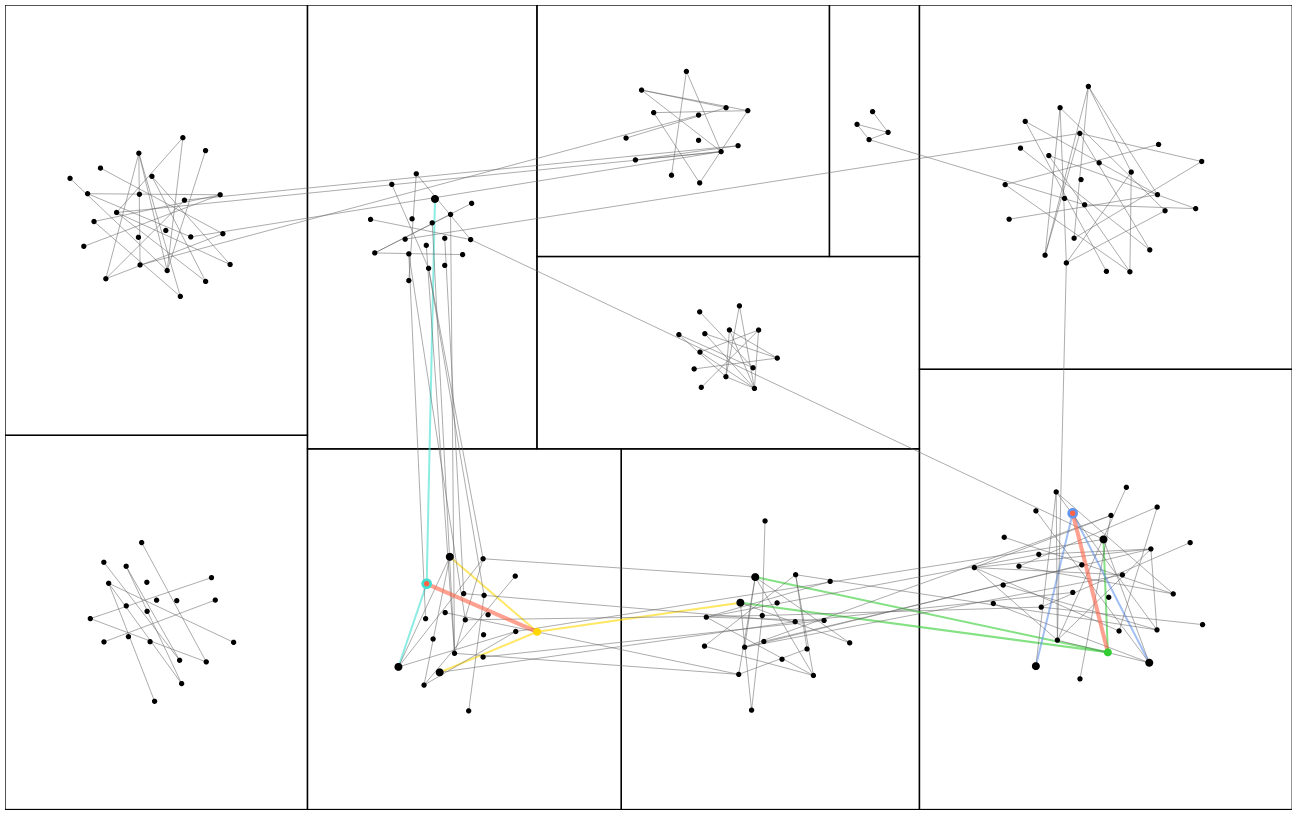
\includegraphics[width=15cm]{./images/ex2-screenshot.png}
  \caption{実験2のスクリーンショット。ネットワーク内の2点が赤く与えられ、これらを繋ぐパスを探索する。}
  \label{fig:screenshot-ex2}
  \end{center}
\end{figure}

\section{実験に用いたデータ}
\label{sec:data_ex2}
本節では実験2に用いたデータについて記述する。
データの生成法は実験1と同じであるが、本実験ではデータの大きさを実験での関心変数とすることから、いくつかの点を変更している。
以下では主にその変更点について二章に分けて述べる。

\subsection{データサイズ}
\label{subsec:data_size}
本実験では、FD-GIBとTR-GIBのデータ拡張性を調べるために、2種類のデータサイズのネットワークを用いる。
データサイズとは主にノード、リンク、グループの数により決まるものであるが、今回はグループの数のみを変数とする。
これは、GIBの特性を考慮したためである。
各GIBの差異はグループの配置と箱の形により生まれるものであり、レイアウトの外形はグループの数に最も左右されうる。
ノードやリンクの数を変えてもレイアウトの外形は大きく変わらないため、グループの数を変えることでレイアウトのデータ拡張性が明らかになると考えた。
言い換えれば、グループの数によりレイアウトの有効性が決定され、ノードやリンクの数の増減は有効性に大きく影響しないということである。
以上の理由より、本実験ではグループの数を10と40に固定する。
同様にノードの数は実験1を参考に$V_{\text{mean}} = 20, V_{\text{stdev}} = 10$とした。

\subsection{データの特徴}
\label{subsec:data_feature}
実験1とは異なり、本実験ではグループのサイズを10と40とで変化させる。
グループの数が10ほどの時は実験1と同じパラメータでデータ生成をしても問題なかったが、グループの数が40ともなるとタスクを行うにはリンクの数が多すぎることが分かった。
これは現実のネットワークを考慮すると自然なことである。
例えばユーザーがノード、フォロー関係がエッジとして表されるTwitterのネットワークを考える。
住んでいる国のような特定のグループ内ではノード(ユーザー)同士の関係は密であると考えられる。
しかし、グループの数が増えたからと言って、国内と同じ割合で国外のユーザーと繋がるわけではないのである。
このことを考慮すると、グループの数が増えた時は他のグループとの関わりう確率を下げてデータを生成する必要がある。

Yoghourdijianらは、グラフ描画の手法のユーザー実験に関する調査論文を発表している\cite{yoghourdjian2018exploring}.
その中で、彼らはタスク結果に影響する視覚的複雑さを紹介しているが、その中でエッジの密度という指標が非常に重要だと述べている。
エッジの密度はノードの数に対するエッジの数の割合として定義される。
密度を表す式はエッジに数を$|E|$、ノードの数を$|N|$とした時、
\[
  \text{density} = \frac{|E|}{|V|(|V| - 1)},  \text{linear density} = \frac{|E|}{|N|}
 \]
の2種類があり、これらは使用用途に合わせそのどちらもが使用可能で、これが変化するとグラフの可読性が大きく左右されるとYoghurdijianらは述べている。
本実験では可用性を考慮しlinear densityを密度として用い、グループの数が異なる時でもエッジの密度を一定にするデータ生成法をとった。

\ref{subsec:data_algorithm}項で述べた我々のデータ生成法では、エッジの数$|E|$は以下のように表される。
\[
  |E| = V_{\text{mean}} m p_{\text{in}} + V_{\text{mean}}^2 + m^2 p_{\text{group}} p_{\text{bridge}} + V_{\text{mean}}^2 m^2 p_{\text{out}}
\]
ここで、$m$はグループの数である。
ノードの数は$m V_{\text{mean}}$と表されるので、密度は以下の式のように表せる。
\[
  \text{density} = p_{\text{in}} + V_{\text{mean}} + m p_{\text{group}} p_{\text{bridge}} + V_{\text{mean}} m p_{\text{out}}
\]
これが$m$に依らず一定となるように$p_{\text{in}}, p_{\text{group}}, p_{\text{bridge}}, p_{\text{out}}$を定めればよい。
エッジの生成確率を定めるため、密度以外にもう一つ、以下の式で表される外部リンクの数に対する内部リンクの数の割合を考慮した。
\[
  \frac{p_{\text{in}}}{m (p_{\text{group}} p_{\text{bridge}} + p_{\text{out}})}
\]
これを一定にすることで、実験に用いるデータを均質化することができる。

密度と内部リンクの割合が一定になるように、以下のように値を制御した。
\[
  p_{\text{in}} = 0.075, p_{\text{group}} = \frac{0.57}{m}, p_{\text{bridge}} = 0.02, p_{\text{out}} = \frac{0.0057}{m}
\]
この時密度は1.5, 内部リンクの割合は4.4となり、密度はYoghourdijianら\cite{yoghourdjian2018exploring}が報告した調査対象の論文で用いられた各グラフの密度の中央値に一致する。
内部リンクの割合はChaturvediら\cite{chaturvedi2014group}が報告したTwitterデータの平均値である3.8に近い。
これらの値を制御することで、グループの大きさに依らず現実のものに近いデータを生成した。

\subsection{最短パスの設定}
\label{subsec:shortest_path}
データ生成の際、ネットワークの中から2ノードを選ぶタスクの答えとなる最短パスを設定した。
どの2ノードを選ぶかはタスクの難易度を大きく左右するため、非常に重要である。
実験の信頼性を確保するため、我々はどの刺激でも等しい難易度になるようにこれを調整した。
2ノードを$n_1, n_2$とする時、その手法は以下である。
\begin{enumerate}
  \item $n_1$からノードを重複せずに5, 7ノードでたどり着けるノードの集合を$S_5^1, S_7^1$とする。
  \item $S_5^1$と$S_7^1$の両方において、$n_2$の割合が2\% - 3\%の範囲に収まるような$n_1, n_2$を選択する。
  \item $n_2$からも同様に$S_5^2, S_7^2$を計算し、$n_1$の割合が2\% - 3\%の範囲に収まるよう$n_1, n_2$を選択する。
\end{enumerate}
この方法により、$n_1, n_2$どちらから探索した時も、すべての刺激において難易度が一定になるように調整した。


\section{仮説}
\label{subsec:hypothesis-ex2}
実験2で検証する仮説は以下の2つである。
\begin{description}
  \item{\bf 仮説1.} グループの数が10の時、FD-GIBがTR-GIBよりも正答率が高い。
  \item{\bf 仮説2.} グループの数が40の時、TR-GIBがFD-GIBよりも正答率が高い。
\end{description}
これらの仮説は実験1の結果に加え各レイアウトにおける箱の大きさを考慮し立てられた。
グループ数が10の時、FD-GIBの各箱の大きさはタスクを行うのに十分であり、また外部リンクを箱の外に描くことによりトポロジーの可読性が高いことから、FD-GIBの方が良い結果を残すと考える。
TR-GIBはエッジの長さを短くすることにより内部リンクを効果的に描画できるが、実験1のタスク3ではより抽象的な問題においてであったがFD-GIBの方が良い成績を残したことから、グループ数が10の際はFD-GIBに優位性があると考えた。
一方でグループ数が増えると、FD-GIBは箱のサイズが小さくなり内部リンクを認識するのが難しい他、トポロジーを効果的に表示するという機能が弱まると考える。
というのも、FD-GIBで採用しているforce-directedレイアウトは、ノードが多くなると視覚的な複雑さが増し、全体のトポロジーを理解するのが難しくなるからである。
TR-GIBは最適化を行うために、グループ数が多くなってもレイアウトの有効性が保たれるため、40グループではTR-GIBの方が有効だと考える。


\section{実験デザイン}
\label{sec:ex2-design}
本実験は、グループの数毎にレイアウトのみを独立変数とした比較検定を反復測定により行う。
実験1と同様、正規分布に従うノードの数などは考慮しないものとする。

データは10グループと40グループでそれぞれ30問生成し、これに2種類のレイアウトを適用した120問で実験を構成した。
実験1と異なり2レイアウトで同一のデータを用いている。
これは実験内で同一データを見る回数が2回では慣れの影響が少なく、同一データでの手法の違いを議論できる利点の方が大きいと判断したためである。
問題の順番はグループの数に問わずランダム化され、タスクは6ブロックに分かれ20問毎に被験者は休憩を挟んだ。
被験者は視線追跡データを記録する都合上同じ順番で問題に取り組んだ。

被験者の疲労を考慮し各刺激において制限時間は30秒とした。
長時間の実験は被験者に疲労がたまりパフォーマンスが落ちる。
本実験では説明と練習を合わせ1時間半を超えないように制限時間を設けた。

\section{実験の流れ}
実験の流れは実験1と同様である。
簡単なアンケートの後に生体計測、視線追跡、GIBレイアウトに関する説明を行い、生体計測に関する同意書に署名を得た。
各グループの数とレイアウト毎に10問ずつの計40問チュートリアルを行なった後、本実験を行なった。

本実験では、被験者は20問毎に数分の休憩を挟みタスクに取り組んだ。
被験者には最短パスに拘らず、問題を早く解くことに努めるよう促した。
正解のパスを選ぶとそれがピンク色で色付けされ、スペースキーを押すことで次の問題へと移行する。
制限時間になるとスクリーンからグラフが消え、画面が白くなる。
同様にスペースキーを押すことで次の問題が現れる。

本実験は実験1と同様に人工照明で照らされた簡素な部屋で行われ、携帯電話は電源をオフにした。
ディスプレイは解像度$2560 \times 1440$のものを用い、被験者の顔は画面から65cmの位置に顎台をもって固定した。
視線追跡データはTobii Pro X3-1120により録画し、眼球運動の判定にはI-VTフィルター\cite{olsen2012tobii}を用いた.

\section{被験者}
被験者は可視化を学ぶ京都大学の学生と教員の計14人で、13人が男性、1人が女性であった。
3名が日本人で残りが中国人で、どちらの国でも文章を左から右に、上から下に読む。
被験者は全員正常もしくは矯正された視力を有した。
実験時間は休憩を含み1時間半ほどであった。

\section{結果}
\label{sec:result-ex2}
本章では実験2の結果について記述する。
実験1と同様、解答の正否と完了時間、そして視線追跡データが計測された。
正答率と完了時間に対しては、Wilcoxonの符号順位検定を用いて2群間に有意差があるかを判定した。
また実験には制限時間が設けられており、完了時間は最大で30秒となったために、正当時の完了時間も同様に差を検討した。
この際はデータに対応関係がないためMann-WhitneyのU検定を用いた。
全ての検定で有意確率$p$は$p = 0.05$とした。

グループ数が10の時、FD-GIBの平均正解率は63.6\%, TR-GIBの平均正解率は69.8\%であった。
Wilcoxonの符号順位検定より、正答率 ($p=0.026$)と完了時間($p=0.006$)において有意差が見られ、TR-GIBの方がどちらにおいても優秀な成績を残した。
一方で、正当時の完了時間に有意差は見られなかった。
平均値の差はTR-GIBの方が正答率が6.2\%高く、完了時間が1374ms早かった。

グループ数が40の時、FD-GIBの平均正答率は56.4\%, TR-GIBでは71.4\%であった。
Wilcoxonの符号順位検定により、正答率($p<0.001$)と完了時間($p < 0.001$)、そしてMann-WhitneyのU検定より正当時の完了時間($p = 0.037$)に有意差が見られ、被験者はTR-GIBにおいてより良い結果を出した。
平均値の差は正答率が15.0\%, 完了時間が2792ms, 正当時の完了時間が1040msであった。

以上の結果より、仮説1.は反駁され、仮説2.は支持された。
グループ数によらずTR-GIBの方が高い正答率を残したが、グループ数が40の時の方が2レイアウト間の正答率の差は大きくなった。
また、同じデータを用いた時でのレイアウト間での正答率の相関係数は、グループ数が10の時$0.768$, グループ数が40の時$0.595$とどちらも比較的強い相関関係が見られた。

\begin{figure}[t]
  \begin{center}
  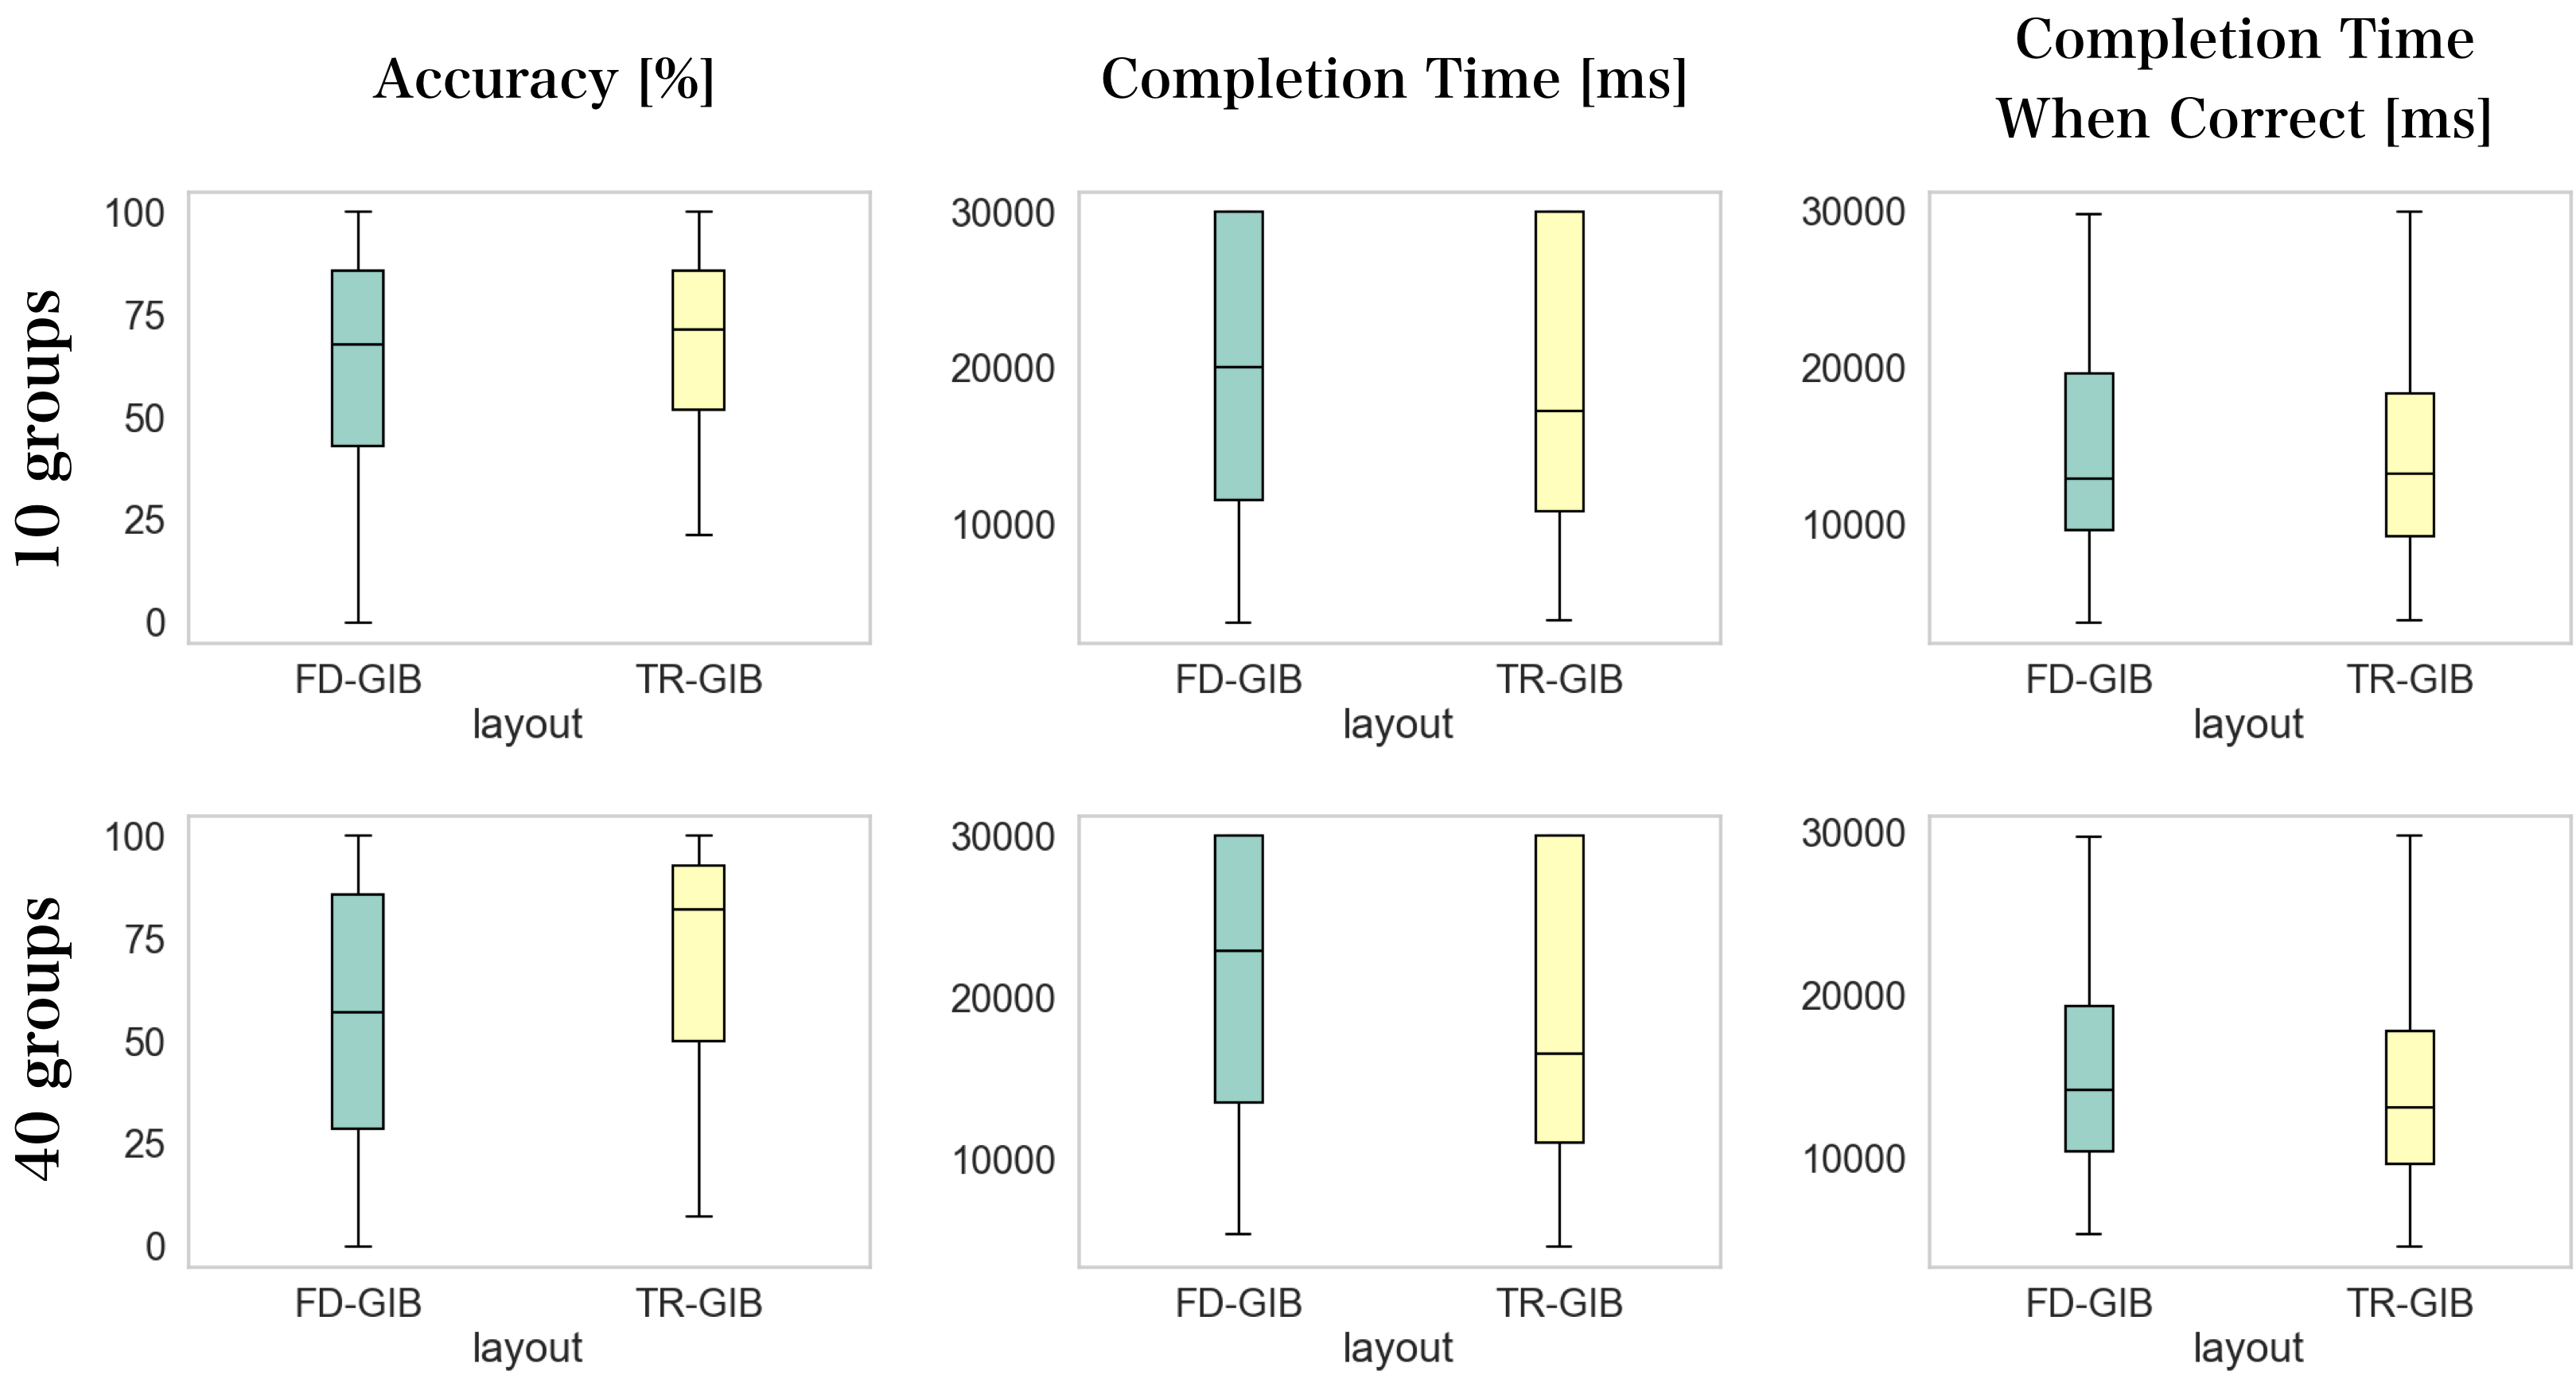
\includegraphics[width=15cm]{./images/ex2-result.png}
  \caption{実験2の結果。左から正答率、完了時間、正当時の完了時間をグループの数ごとに示している。}
  \label{fig:screenshot-ex2}
  \end{center}
\end{figure}

\section{考察}
本節では実験結果に対し考察を与える。
主に、各グラフにおけるどの視覚特徴がタスクにおける効果に差を生んだのかを視線追跡データに基づいて議論する。

\subsection{被験者の行動の分類}
本実験で用いた完了に数十秒を要する複雑なタスクはすぐに答えにたどり着けないために、被験者は完了までに部分タスクと呼ばれるいくつかのプロセスを踏むと知られている。
我々は\ref{sec:result-ex2}節で述べた結果がなぜ生まれたのかを議論するため、タスクにおける被験者の行動を視線追跡データを用いて分類し、それぞれの部分タスクでの被験者の行動に注目する。

図\ref{fig:taxonomy}に視線追跡データに基づいた被験者行動の分類図を示す。
我々は視線追跡データを検証するにあたり、注視点が固定されているか多くの場所を見ているかで、被験者行動が大きく二分されていることを確認した。
これを定量的に評価するため、各刺激に対する各被験者の視線データを始点と終点を合わせ、線形に15のセグメントに分割し、それぞれのセグメントにおいて何回注視するAOIを変化させたか(注視したAOIの数)と注視したAOI(注視したAOIの種類)が何種類あるかを計算した。
ここで、AOIは実験1同様に各ボックスと一致するように定義される。
図\ref{fig:taxonomy}は、これらの指標と時間(0が始点)に対して、記録した全視線データのうちどれだけのセグメントが一致したかを示している。
例えば、図\ref{fig:taxonomy} (a) のFD-GIBでは、刺激中のどのタイミングでいくつのAOIが注視されていたかをヒートマップで示している。
ヒートマップにおいて色が濃い点は、被験者がそのタイミングでその数のAOIを頻繁に注視していたことを表し、色の薄い点はそのタイミングではその数のAOIを注視していなかったことを表す。

我々は、各ヒートマップにおいて大きくトレンドが分かれる点を視覚的に判別し、それにより行動を分類し図\ref{fig:taxonomy}では色の異なる箱で囲っている。
図\ref{fig:taxonomy} (a) では、注視したAOIの数が5か6かでトレンドが分かれると判断した。
図\ref{fig:taxonomy} (b) では、注視したAOIの種類が2か3かでトレンドが分かれると判断した。
図\ref{fig:taxonomy} (c) では、注視したAOIの数と種類がどちらも少ないとき、数の方が種類より多い時、種類が2より多い時で異なるトレンドがあると判断し分類した。
また、被験者の行動は刺激の開始直後と終了の直前で異なると考えたため、図\ref{fig:taxonomy} (a) では前半と後半で行動を分類している。
それぞれの図において注視したAOIの数が0のセグメントでは、眼球が断続性運動をしていると判断されるためこれも別の分類にしている。
また、それぞれの分類の色は各図においての分類番号に即したものであり、図\ref{fig:taxonomy} (a)と図\ref{fig:taxonomy} (b)の色は対応したものでは無い。

このデータには3種類の効果が考えられる。
一つは、FD-GIBの箱の大きさである。
箱が小さいために注視の数が増える。
二つ目は、セグメントに分けたことである。
早く終わった刺激では注視の数が少なく、長くかかったものでは注視の数が多い。

記録した全視線データの中で、各分類に含まれるセグメントの数を計算した。
部分タスクの分類は計9つに分かれ、それを以下に示す。
\begin{description}
  \item{分類0.} 眼球の断続性運動。
  \item{分類1.} 前半のセグメント。注視AOIの数も種類も少ない。
  \item{分類2.} 前半のセグメント。注視AOIの数は少ないが種類は多い。
  \item{分類3.} 前半のセグメント。注視AOIの数は多いが種類は少ない。
  \item{分類4.} 前半のセグメント。注視AOIの数も種類も多い。
  \item{分類5.} 後半のセグメント。注視AOIの数も種類も少ない。
  \item{分類6.} 後半のセグメント。注視AOIの数は少ないが種類は多い。
  \item{分類7.} 後半のセグメント。注視AOIの数は多いが種類は少ない。
  \item{分類8.} 後半のセグメント。注視AOIの数も種類も多い。
\end{description}
また図\ref{fig:taxonomy-result}はレイアウト、グループ数、解答の正否ごとに各分類でのセグメントの数を表したものである。
この図においての各レイアウトの差が、それぞれの部分タスクにおける被験者の行動の差と言える。

4と8が主にこの差を生む。
3と7が10グループで間違いの時。




\begin{figure}[t]
  \begin{center}
  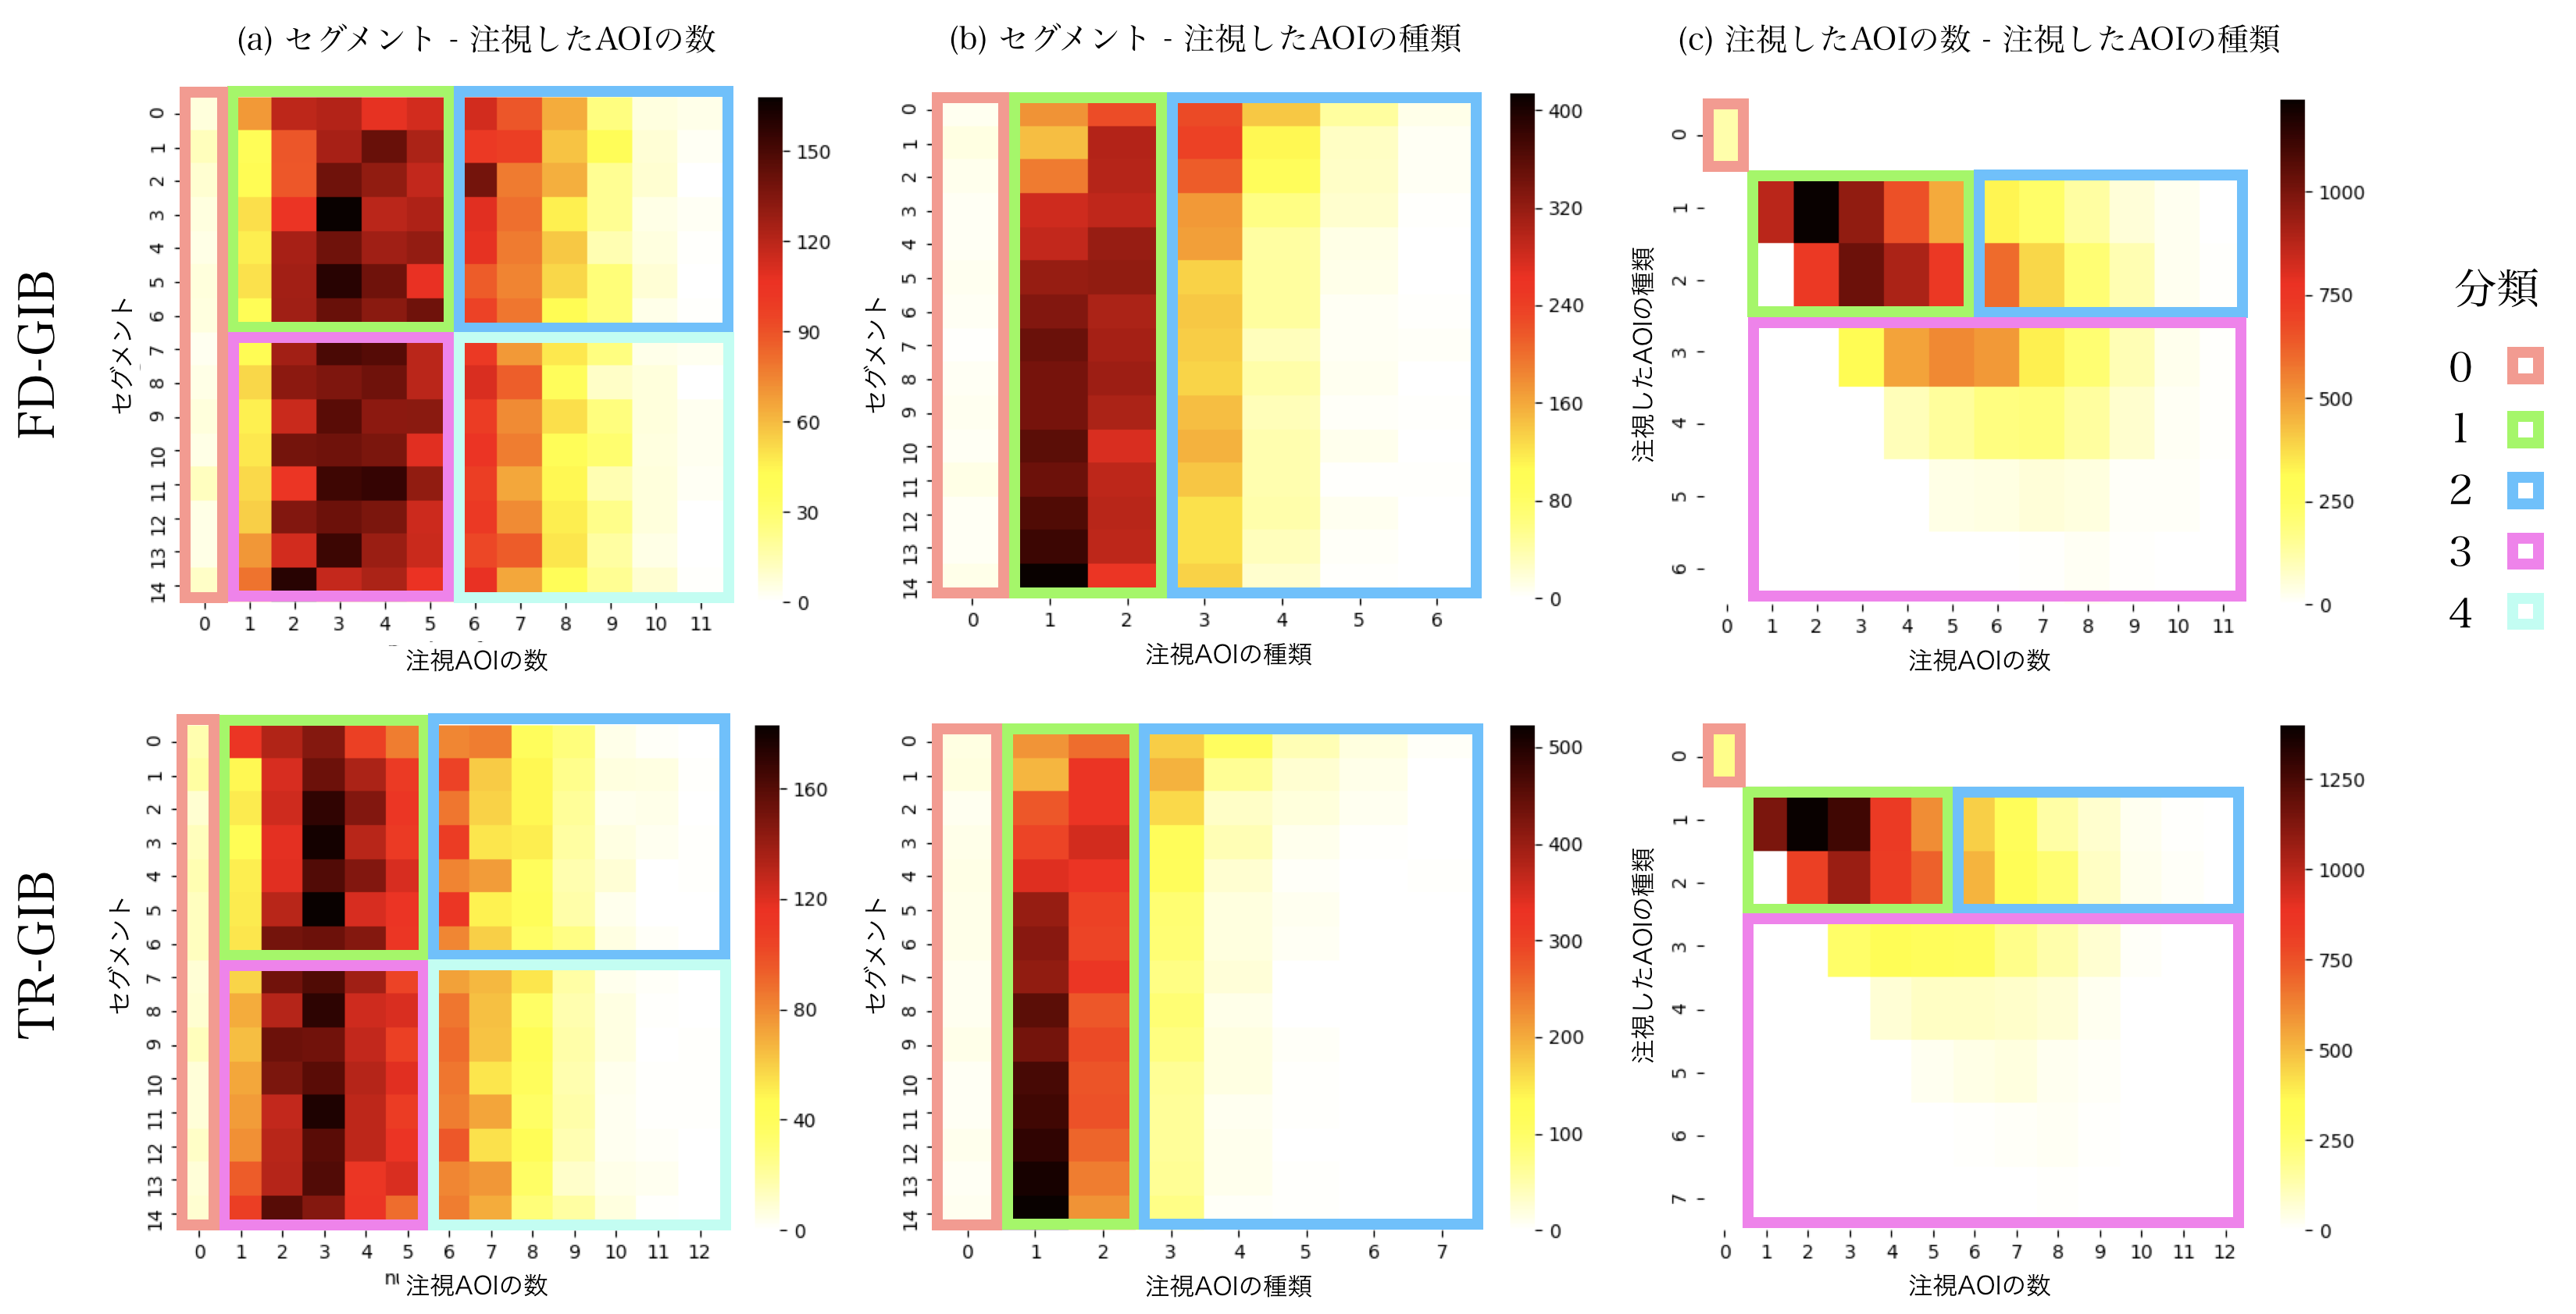
\includegraphics[width=15cm]{./images/taxonomy.png}
  \caption{}
  \label{fig:taxonomy}
  \end{center}
\end{figure}

\begin{figure}[t]
  \begin{center}
  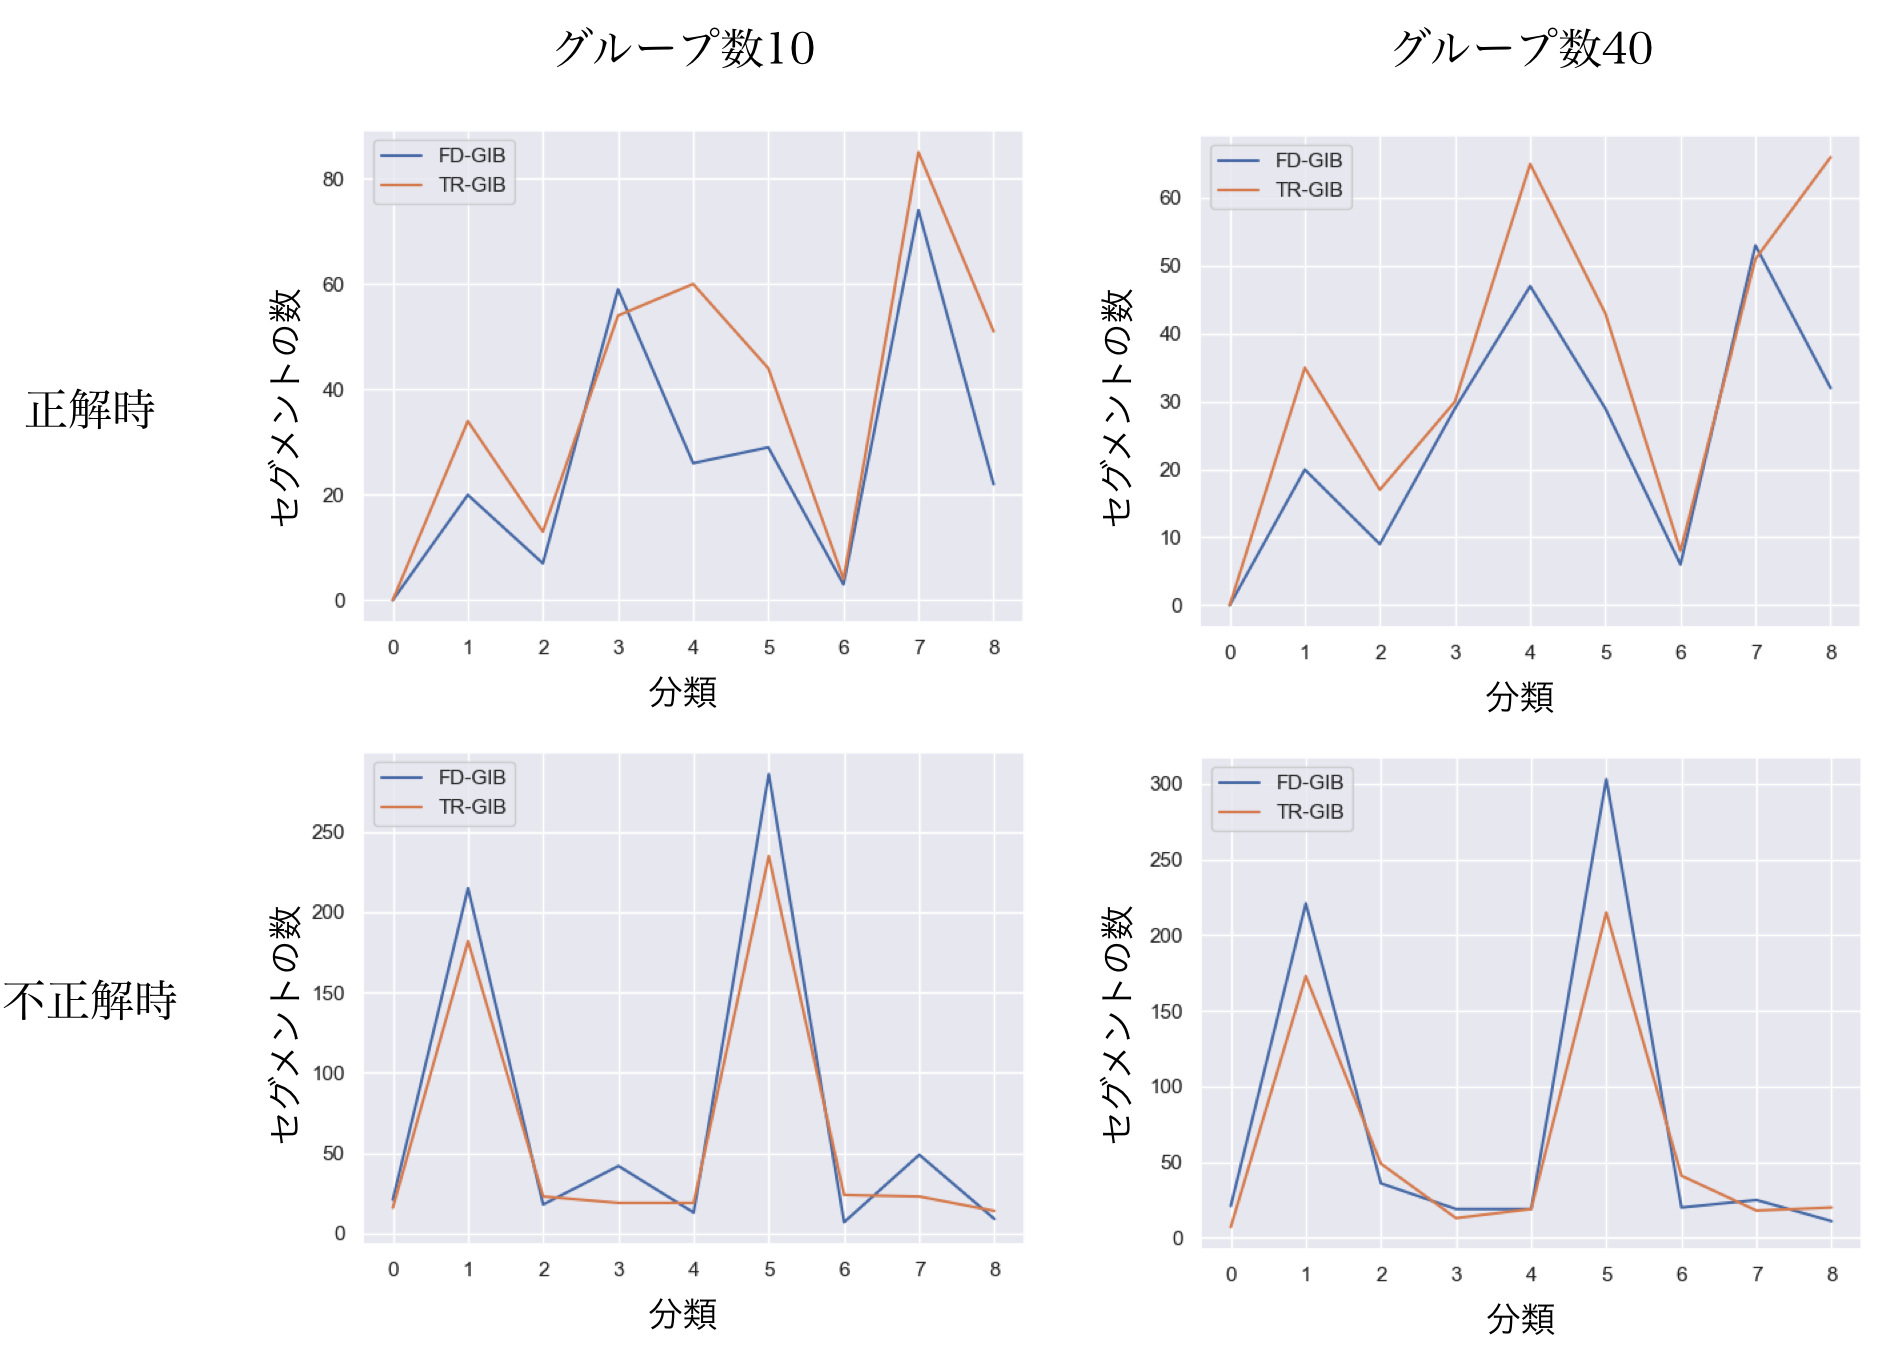
\includegraphics[width=15cm]{./images/taxonomy-result.png}
  \caption{}
  \label{fig:taxonomy-result}
  \end{center}
\end{figure}








\section{GIBを提供するWebサイト}

%======================================================================
%   謝辞
%======================================================================
\begin{acknowledgements}

\end{acknowledgements}



%======================================================================
%   参考文献
%======================================================================
\bibliographystyle{kueethesis}
\bibliography{sample}



%======================================================================
%   付録
%======================================================================
\appendix

\end{document}
% Local Variables:
% fill-column: 70
% End:
